\documentclass[12pt]{article}
\usepackage{graphicx,psfrag,float,mathbbol,xcolor,cleveref}
\usepackage{arydshln}
\usepackage{amsfonts}
\usepackage{amsmath}
\usepackage{tikz}
\usepackage[mathscr]{euscript}
\usepackage[utf8]{inputenc}
\usepackage[english]{babel}
\usepackage{natbib} 
\usepackage[T1]{fontenc}
\usepackage{enumitem}
\usepackage{accents}
\usepackage{bm}
\usepackage{framed}
\usepackage{subcaption}
\usepackage{mathtools}
\usepackage{IEEEtrantools}
\usepackage{times}
\usepackage{amsthm}
\usepackage{tabularx,ragged2e,booktabs,caption}


\newcolumntype{C}[1]{>{\Centering}m{#1}}
\renewcommand\tabularxcolumn[1]{C{#1}}
\usepackage[letterpaper, left=1in, top=1in, right=1in, bottom=1in,nohead,includefoot, verbose, ignoremp]{geometry}
\newcommand{\comment}[1]{\text{\phantom{(#1)}} \tag{#1}}
\newcommand{\ms}{\scriptscriptstyle}
\newcommand\numberthis{\addtocounter{equation}{1}\tag{\theequation}}
\newcommand*\needsparaphrased{\color{red}}
\newcommand*\needscited{\color{orange}}
\newcommand*\needsproof{\color{blue}}
\newcommand*\outlineskeleton{\color{green}}
\newcommand{\PP}{\mathcal{P}}
\newcommand{\R}{\mathbb{R}}
\newcommand{\bfeps}{\mbox{\boldmath $\epsilon$}}
\newcommand{\bfgamma}{\mbox{\boldmath $\gamma$}}
\newcommand{\bflam}{\mbox{\boldmath $\lambda$}}
\newcommand{\vphistar}{\mbox{\boldmath $\phi^*$}}
\newcommand{\vsigmasq}{\mbox{\boldmath $\sigma^2$}}
\newcommand{\bfbeta}{\mbox{\boldmath $\beta$}}
\newcommand{\bfalpha}{\mbox{\boldmath $\alpha$}}
\newcommand{\bfe}{\mbox{\boldmath $e$}}
\newcommand{\bfone}{\mbox{\boldmath $1$}}
\newcommand{\bft}{\mbox{\boldmath $t$}}
\newcommand{\bfo}{\mbox{\boldmath $0$}}
\newcommand{\bfO}{\mbox{\boldmath $O$}}
\newcommand{\bfx}{\mbox{\boldmath $x$}}
\newcommand{\bfX}{\mbox{\boldmath $X$}}
\newcommand{\bfz}{\mbox{\boldmath $z$}}


\newcommand{\bfl}{\mbox{\boldmath $l$}}
\newcommand{\bfm}{\mbox{\boldmath $m$}}
\newcommand{\bfy}{\mbox{\boldmath $y$}}
\newcommand{\bfa}{\mbox{\boldmath $a$}}
\newcommand{\bfb}{\mbox{\boldmath $b$}}
\newcommand{\bfY}{\mbox{\boldmath $Y$}}
\newcommand{\bfS}{\mbox{\boldmath $S$}}
\newcommand{\bfZ}{\mbox{\boldmath $Z$}}
\newcommand{\cardT}{\vert \mathcal{T} \vert}

\newtheorem{theorem}{Theorem}[section]
\newtheorem{lemma}[theorem]{Lemma}
\newtheorem{proposition}[theorem]{Proposition}
\newtheorem{corollary}[theorem]{Corollary}

\theoremstyle{definition}
\newtheorem{definition}{Definition}[section]
\newtheorem{example}{Example}[section]
\def\bL{\mathbf{L}}


\makeatletter
\renewcommand{\theenumi}{\Roman{enumi}}
\renewcommand{\labelenumi}{\theenumi.}
\renewcommand{\theenumii}{\Alph{enumii}}
\renewcommand{\labelenumii}{\theenumii.}
\renewcommand{\p@enumii}{\theenumi.}
\makeatother

\bibliographystyle{abbrvnat}


\begin{document}


\title{ Nonparametric Covariance Estimation for Longitudinal Data via Penalized Tensor Product Splines}

\author{Tayler A. Blake\thanks{The Ohio State University, 1958 Neil Avenue, Columbus, OH 43201} \and  Yoonkyung Lee\thanks{The Ohio State University, 1958 Neil Avenue, Columbus, OH 43201}}

\maketitle

\begin{abstract}
With high dimensional longitudinal and functional data becoming much more common, there is a strong need for methods of estimating large covariance matrices. Estimation is made difficult  by the instability of sample covariance matrices in high dimensions and a positive-definite constraint we desire to impose on estimates. A Cholesky decomposition of the covariance matrix allows for parameter estimation via unconstrained optimization as well as a statistically meaningful interpretation of the parameter estimates. Regularization improves stability of covariance estimates in high dimensions, as well as in the case where functional data are sparse and individual curves are sampled at different and possibly unequally spaced time points. By viewing the entries of the covariance matrix as the evaluation of a continuous bivariate function at the pairs of observed time points, we treat covariance estimation as bivariate smoothing. 

Within regularization framework, we propose novel covariance penalties which are designed to yield natural null models presented in the literature for stationarity or short-term dependence. These penalties are expressed in terms of variation in continuous time lag and its orthogonal complement. We present numerical results and data analysis to illustrate the utility of the proposed method. \\
\\
%\begin{keywords}
{\bf keywords:} non-parametric, covariance, longitudinal data, functional data, splines, reproducing kernel Hilbert space
%\end{keywords}
\end{abstract}

\section{Introduction}

Covariance estimation with high dimensional data has has recently gained growing interest; it is generally recognized that there are two primary hurdles responsible for the difficulty in covariance estimation: the instability of sample covariance matrices in high dimensions and a positive-definite constraint we wish estimates to obey. Estimation of population covariance matrices from samples of multivariate data has been important for methods in classical multivariate data analysis, time series analysis, spatial statistics and, more recently, the growing field of statistical learning. Covariance estimates play a critical role in establishing independence or conditional independence through graphical models, constructing discriminant functions as in linear discriminant analysis (LDA) and quadratic discriminant analysis (QDA) for the classification of Gaussian data, building confidence intervals for component means and contrasts, and constructing a low-dimensional representation of data via principal components analysis (PCA). One may note that the last two techniques require an estimate of the covariance matrix, and the first two require estimation of the inverse.

Prevalent technological advances in industry and many areas of science make high dimensional longitudinal and functional data a common occurrence, arising in numerous areas including medicine, public health, biology, and environmental science with specific applications including fMRI, spectroscopic imaging, gene microarrays among many others, presenting a need for effective covariance estimation in the challenging situation where parameter dimensionality is possibly much larger than the number of observations. Additional difficulty due to constraints required to yield positive definite estimates make covariance estimation a potentially complex optimization problem. Further, most existing approaches to covariance estimation require data to be sampled at regular grid (time) points, with subjects sharing a set of common observation points. However, in many practical situations, data are irregularly sampled, and subjects may share few common observation times, and methods are needed to accommodate for data collected in this way.  

To address the challenge of enforcing positive definiteness, several have considered modeling various matrix decompositions including variance-correlation decomposition, spectral decomposition, and Cholesky decomposition. The Cholesky decomposition has received particular attention, as it which allows for a statistically meaningful interpretation as well as an unconstrained parameterization of elements of the covariance matrix. This parameterization allows for estimation to be accomplished as simply as in least squares regression. 



It is well known that the sample covariance matrix is unstable in high dimensions, and there is an extensive existing body of work addressing the issue of high dimensionality in the context of covariance estimation. See \citet{pourahmadi2011covariance} for a survey of approaches to covariance estimation from the generalized linear modeling and regularization perspectives. However, much of this work addresses high dimensionality arising from functional or times series data sampled on a dense, regular grid. With such data, it is typical that the number of time points is larger than the number of observations. Few have addressed the challenges posed by sparse longitudinal data where measurement times may be almost unique yet sparsely distributed within the observed time range for each individual in the study. In this case, high dimensionality may not be a consequence of having more measurements per subject than the number of subjects themselves, but rather because when pooled across subjects, the total number of unique observed time points is greater than the number of individuals. Incomplete and unbalanced data arise when measurement schedules with targeted time points which are not necessarily equally spaced or if there is missing data. Sparse longitudinal data arise when the measurement schedule has arbitrary or almost unique time points for every individual. A given time point may have very few individuals with corresponding measurements. 

We sidestep both issues of high dimensionality and irregularly sampled data by viewing the response as a stochastic process having continuous covariance function. Recent work outlines the use of function estimation for smoothing elements of the covariance matrix, including \citet{wu2003nonparametric},\citet{huang2007estimation}. To our knowledge, however, no previous work has applied  smoothing to both dimensions of the Cholesky factor;  we model the generalized autoregressive parameters using tensor product splines. Viewing covariance modeling as bivariate function estimation both accommodates irregularly sampled curved and permits interpolation and extrapolation of the covariance function between two measurements at any pair of time points within the time interval of interest rather than at observed pairs of time points only. The Cholesky decomposition enables covariance estimation through the estimation of a varying coefficient model. A transformation of the design point axes allows for an ANOVA-like decomposition of the coefficient function into two components, corresponding to the lag between time points and an additive component. Through this general framework, we can easily impose penalties on fitted functions to yield natural null models presented in the literature. 

\section{Cholesky Decomposition of $\Sigma$}

To present a comprehensive overview our estimation procedure, we begin with the representation of the inverse covariance matrix, $\Omega = \Sigma^{-1}$, in terms of its Cholesky decomposition (see \citet{pourahmadi2007cholesky} for a detailed discussion.) In the section to follow, we will demonstrate that this parameterization of the precision matrix is particularly attractive due to both the computational advantages as well as the convenient modeling interpretation it permits. For any positive definite matrix $\Sigma$, there exists a unique unit lower triangular matrix $T$ with diagonal entries equal to $1$ which diagonalizes $\Sigma$:

\begin{equation}
\nonumber T \Sigma T^\prime = D
\end{equation}
\noindent

If we assume that the data having covariance matrix $\Sigma$ follow an autoregressive model, then the entries of the Cholesky factor $T$ and $D$ enjoy a useful interpretation. Let $Y = \left( Y_{1}, Y_{2}, \dots, Y_{m} \right)^\prime$ be defined on a probability space with some probability measure $\mathcal{P}$ corresponding to the multivariate Normal distribution with mean $0$ and covariance $\Sigma$, and let $Y_1,Y_2,\dots, Y_m$ have associated measurement times 

\[
t_{1} < t_{2} < \dots< t_{m}.
\]


Let $\hat{y}_t$ denote the linear least-squares predictor of $y_t$ based on its predecessors $y_1,\dots, y_{t-1}$, and let $e_t$ denote its prediction error with variance $Var\left(e_t\right)=\sigma_t^2$, $Cov\left(e_i,e_j\right)=0$ for $i \ne j$. Standard regression theory gives us that we can find coefficients $\phi_{tj}$ such that

\begin{equation}
{y}_{j}  = \sum_{k=1}^{j-1} \phi_{jk} y_{k} + \sigma_{j}e_{j}, \qquad j=2,\dots,m, \label{eq:ARmodel}.
\end{equation}

Let $T$ denote the $m \times m$ unit lower triangular matrix with elements 

\[
T_{jk} = \left\{
\begin{array}{ll}
-\phi_{jk} & j > k\\
1 & j = k \\
0 & otherwise,
\end{array}\right.
\]
\noindent
for $j,k=1,\dots,m$. In matrix notation,  model~\ref{eq:ARmodel} may then be written

\begin{equation}
e = T Y, \label{eq:epsilon}
\end{equation}
\noindent

Taking covariances on both sides of \ref{eq:epsilon}, we have

\begin{equation} \label{eq:cholesky_decomp}
D = T \Sigma T^\prime
\end{equation} 

An attractive feature of this reparameterisation is that, regardless of the modelling approach, the estimated covariance matrix is guaranteed to be positive definite. The unconstrained regression coefficients $\lbrace \phi_{jk} \rbrace$ are referred to as the \emph{generalized autoregressive parameters} (GARPs). The $\lbrace \sigma^2_{j} \rbrace$ are called the \emph{innovation variances} (IVs.)  Unconstrained estimation of the $\left\{ \sigma_{k}^2 \right\}$ is achieved by log transformation;  we leave these details for section 2. Expressing the precision matrix  in terms of the GARPs and IVs, we have
\begin{equation*} \label{eq:omega_decomp}
\Omega= \Sigma^{-1} = T^\prime D^{-1} T.
\end{equation*}

Rather than estimating a specific covariance matrix for data observed on a fixed, regular grid, we aim to estimate a smooth covariance function. This accomodates data which may consist of  observations on multiple subjects measured at potentially unequally spaced and individual-specific times. In estimation of the means $\mu$ of p-vectors of i.i.d. variables, the
Gaussian white noise model [9] is the appropriate infinite-dimensional model into
which all objects of interest are embedded. In estimation of matrices, a natural
analogue is the space B(l2,l2), which we write as B, of bounded linear operators
from l2 to l2. These can be represented as matrices [cite \textit{Regularized estimation of large covariance matrices by Bickel and Levina - section 4.}]

Rather than $m$-dimensional vectors, consider $Y$ and $e$ as the values of the stochastic processes $Y\left(t\right)$ and $e\left(t\right)$ at the set of observation times.  We assume that $Y\left(t\right)$ is equipped with covariance function $G\left(s,t\right)$, and
\[
e\left(s\right) \sim \mathcal{N}\left(0,1\right)
\] 
is a zero mean Gaussian process with unit variance. We assume that $G\left(s,t\right)$ satisfies some smoothness conditions, where smoothness is defined in terms of square integrability of certain derivatives. [TODO: clean up statement about smoothness of covariance function; integrability of covariance function of a stochastic process?] The entries of $\Sigma$, then, correspond to $G$ evaluated at the distinct pairs of observed time points. Similarly, we treat the elements of the precision matrix $\Omega$ as the evaluation of some smooth function, $\omega\left(s,t\right)$.


Viewing the elements of $D$ and the elements of the Cholesky factor $T$ as the evaluation of smooth functions $\sigma\left(\cdot\right)$ and $\phi^*\left(\cdot,\cdot\right)$ leads us to the varying coefficient (VC) models first introduced in the seminal work of Hastie and Tibshirani.  The procedures presented by \citet{fan2000two} and \citet{huang2002varying} utilize varying coefficient models for modeling the mean of longitudinal data; parameterizing the covariance matrix according to \ref{eq:cholesky_decomp} allows us to exploit these models in covariance estimation for such data as well.  A generalization of traditional linear regression models, varying coefficient models offer more flexibility than their static analogues by allowing the effect of covariates to change smoothly with the value other variables. Both regressors and response variables are assumed to vary according to an \emph{indexing variable}, which  permits interpolation of regressors and response variables at values of this indexing variable where there is either missing data of only a single observation and slope estimation is not feasible.  Replacing  $\left \{ \phi_{jk} \right\}$ and $\left\{ \sigma_j \right\}$ with smooth functions, we model 

\begin{equation}   
y\left(t_j \right)  = \sum_{k=1}^{j-1} \phi\left(t_j ,t_k\right) y\left(t_k\right) + \sigma\left(t_j\right)\epsilon\left({t_j}\right) \;\;\;\; j=1,\dots, m, 
\label{eq:MyModel} 
\end{equation}
\noindent for $t_1 < t_2 < \dots < t_m$. 

%% ASSUMPTIONS ON Y(t): twice differentiable stochastic process on [0,1]

We represent the varying coefficient function and the innovation variances using tensor product smoothing splines and penalized tensor product B-splines. By appending penalties to the negative log likelihood, we can seamlessly control the fit of $\phi$ and $\sigma^2$  to produce final covariance estimates exhibiting the desired null structure.Recasting the problem as the estimation of model~\ref{eq:MyModel} allows us access to the existing set of tools developed in the bivariate smoothing literature; our approach provides a flexible, comprehensive framework for covariance estimation.


\section{Estimating $\phi$ via penalized maximum likelihood}

We employ maximum likelihood  for the estimation of  the varying coefficient function $\phi\left(t,s\right)$ and the innovation variance function $\sigma\left(t\right)$, though neither the derivation the form of model~\ref{eq:ARmodel} nor model~\ref{eq:MyModel} via the Cholesky decomposition rely on any assumptions about the distribution of $Y$. 

For fixed $\left\{ \sigma_j^2 \right\}$, as a function of $\phi_{jk}$ the negative log-likelihood for a sample of $N$  i.i.d. observations $Y_1,Y_2,\dots,Y_N$ from a multivariate Gaussian distribution is proportional to the usual error sums of squares:

\begin{equation}
-2 L\left(y_1,\dots,y_N ,\phi^* \vert \vsigmasq \right) \propto \sum_{i=1}^N \sum_{j=2}^{m_i} \sigma\left({t_j}\right)^{-2} \left(y_{ij} - \sum_{k=1}^{j-1}\phi\left({t_{ij},t_{ik}}\right)y_{ik} \right)^2 \label{loglikelihood}
\end{equation}
\noindent
where 
\[
y_i = \left( y_{i1}, y_{i2}, \dots, y_{i,m_i}\right), \quad i=1,\dots,N 
\] 

%% explain here that we omit y_{i1} from the likelihood here because in the first stage of estimation (for $\phi$), the first observation in each vector doesn't contribute to the likelihood
\noindent
denotes the vector of observations for subject $i$ with corresponding measurement times 
\[
t_{i1} < t_{i2} < \dots < t_{i,m_i}.
\]
The form of the likelihood of $y_1,\dots,y_N$ indicates that we allow both the number of measurements as well as the observation times to varying across subjects. The $\left\{t_{ij} \right\}$ need not be evenly-spaced within or across individuals. Denote the innovation variance function evaluated at the vector of observed time points by $\vsigmasq$, and similarly let $\vphistar$ denote the resulting vector when evaluating $\phi^*$ at the observed grid of time points, transformed to the $l$-$m$ axis. Estimation of the varying coefficient function and the innovation variance function may be accomplished in an iterative fashion:

\fbox{\parbox{\textwidth}{\begin{enumerate}
\item Fix $\vsigmasq = \vsigmasq_0$;
\item find $\widehat{\vphistar} = \underset{\vphistar}{\arg\max} -2 L\left(y_1,\dots,y_N ,\vphistar \vert \vsigmasq_0 \right)$.
\item Fix $\vphistar= \widehat{\vphistar}$;
\item find $\widehat{\vsigmasq} = \underset{\vsigmasq}{\arg\max} -2 L\left(y_1,\dots,y_N , \vsigmasq \vert \widehat{\vphistar} \right)$.
\item Iterate until convergence.
\end{enumerate}}}

\vspace{0.5cm}




% 
%\section{\emph{Penalized maximum likelihood estimation}}
%
%\begin{enumerate}
%\item Fix $\sigma_{ij}^2 = \sigma_{ij0}^2$, $i=1,\dots,N$ ,$j=1,\dots,M$.
%\item Find $\phi_0 = \underset{\phi}{arg \; min} -2L_\phi\left(\phi, y_1,\dots, y_N \right) + \lambda J\left( \phi \right)$
%\item Fix $\phi = \phi_{0}$.
%\item Find  $\sigma_{0}^2 = \underset{\sigma^2}{arg\; min} -2L_\sigma^2\left(\sigma^2, y_1,\dots, y_N \right) + \lambda J\left( \sigma^2 \right)$
%\end{enumerate}
%
%\begin{adjustwidth}{-2cm}{-2cm}
%\begin{equation}
%-2 L_\phi\left(\phi, y_1, \dots,y_N \right) = \sum_{i=1}^N \sum_{j=2}^{m_i} \sigma_{ij0}^{-2} \left(y_{ij} - \sum_{k=1}^{j-1}\phi\left({t_{ij},t_{ik}}\right)y_{ik} \right)^2 \label{loglikelihood}
%\end{equation}
%\end{adjustwidth}
% 





% 
%\section{\emph{Smooth ANOVA models}}
%Decompose
%\begin{equation} \label{eq:SANOVA-model}
%\carrotorangemath{
%\phi^*\left(l,m\right) = \mu + \phi_1\left(l\right) + \phi_2\left(m\right) + \phi_{12}\left(l,m\right)},
%\end{equation} 
%so Model~\ref{eq:MyModel} becomes
%
%\begin{align*}  
%\begin{split}% \label{eq:expanded-ps-anova-vc-model}
% y\left(t_j \right)  = \sum_{k=1}^{j-1} \bigg[\mu + \phi_1\left(l_{jk}\right) +  &\phi_2\left(m_{jk}\right) \bigg.\\[-2ex]
%\bigg. &+ \phi_{12}\left(l_{jk},m_{jk}\right) \bigg]y\left(t_k\right)+ \sigma\left(t_j\right)e\left({t_j}\right)
%\end{split}
%\end{align*}
% 
%

 

%
% \begin{columns}
%\begin{column}{0.5\textwidth}
%Equip $l$ and $m$ with
%\begin{align*}
%B_{1}\left(l\right),\dots, B_{K}\left(l\right),\\
%B_{1}\left(m\right),\dots, B_{L}\left(m\right)
%\end{align*}
%to build
%\begin{equation*}
%T_{jk}\left(l,m\right) = B_j\left(l\right){B}_k\left(m\right)
%\end{equation*}
%  \end{column}
%\begin{column}{0.5\textwidth}  %%<--- here
%    \begin{center}
%    \begin{figure}
%    \graphicspath{{img/}}
% 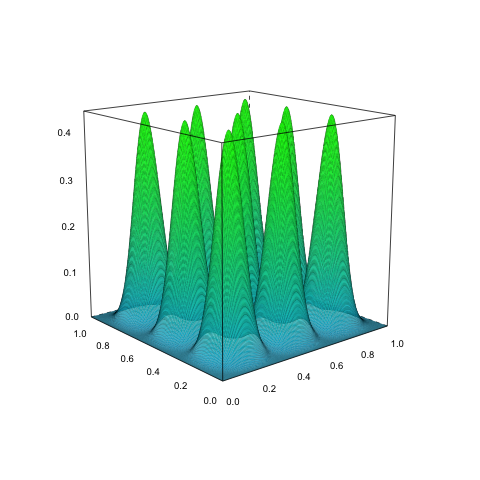
\includegraphics[width=4cm]{sparse_bicubic_basis}
% \caption{A ``thinned'' tensor product basis}
% \end{figure}
%     \end{center}
%\end{column}
%\end{columns}
%\vspace{0.3cm}
%\begin{equation*}
%\phi^*\left(l,m\right) = \sum_{i=1}^K \sum_{j=1}^L \theta_{ij} B_{i}\left(l\right) B_{j}\left(m\right)
%\end{equation*}
%
 



%The parameters of the functional autoregressive model given by \ref{eq:MyModel} define the elements of the precision matrix $\Omega$, rather than the elements of $\Sigma$ itself. It is well known that if we let $Y = \left(Y_1, \dots, Y_m\right)^\prime$ denote the random vector having joint distribution with mean zero and covariance matrix $\Sigma$, then the elements of $\Sigma^{-1}=\Omega$, $\left\{ \omega_{ij} \right\}$ may be interpreted as partial covariances between the elements of $Y$. This suggests shrinking $\phi^*$ to zero for large values of $l$. One can show that if $T$ has $k$ non-zero diagonals, then the middle $k$ diagonals of $\Sigma^{-1}$ are non-zero.  


For ease of exposition, we first focus our attention on the estimation of $\phi$ assume that $\sigma^2\left(t\right)$ is fixed and known. Estimation of the innovation variance function is presented in Section~\ref{section:variance-estimation}. In the case that subjects share a common set of observation times $t_1 < \dots < t_m$,  it is well known that the MLE for $\Sigma$, $S = \sum_{i=1}^N y_i y_i^\prime$ is highly unstable in high dimensions, a condition that is potentially worsened when one or more subjects has at least one observation time that is unique from the set of observation times common across subjects. To mitigate instability due to high dimensionality and simultaneously permit the estimation of $\phi\left(\cdot,\cdot\right)$ as a smooth bivariate function, we obtain a covariance estimator by applying bivariate smoothing of the elements of the Cholesky factor. 

Estimating the varying coefficient function $\phi^*$, however, is quite different from the usual problem of estimating an arbitrary bivariate function. In the case of the latter, we most typically treat both arguments equally in terms of regularization, but in the case of covariance estimation and the generalized coefficient function equal treatment of $l$ and $m$ in terms of penalization perhaps is not the most appropriate approach. The lag component, $l$, has particularly significant meaning in terms of the covariance function and thus also in terms of $\phi^*$ and is of considerable more interest than the orthogonal component, $m$. We parameterize $\phi$ in terms of the transformed domain:

\begin{align*}
l = t-s, \qquad m = \frac{1}{2}\left(s+t\right),
\end{align*}
\noindent
so that the following relationship holds:
\begin{align*}
\phi\left(s,t\right) =\phi^*\left(l,m\right)= \phi^*\left(s-t, \frac{1}{2}\left(s+t\right)\right)
\end{align*}
\noindent
The likelihood can be written in terms of the reparameterized varying coefficient function:

\begin{align} 
\begin{split} \label{loglikelihood}
-2L\left(y_1,\dots,y_N ,\phi^* \vert \vsigmasq \right) &= \sum_{i=1}^n \sum_{j=2}^{m_i} \sigma_{ij}^{-2} \left(y_{ij} - \sum_{k=1}^{j-1}\phi\left({t_{ij},t_{ik}}\right)y_{ik} \right)^2 \\
&= \sum_{i=1}^n \sum_{j=2}^{m_i} \sigma_{ij}^{-2} \left(y_{ij} - \sum_{k=1}^{j-1}\phi^*\left({l_{ijk},m_{ijk}}\right)y_{ik} \right)^2 
\end{split} 
\end{align}

We equip the $l$ and $m$ axes each with a B-spline basis to construct a basis for the varying coefficient function $\phi$ in \ref{eq:phi-star} by taking the tensor product of the two marginal bases. Let 
\[
B_{1}\left(l\right),\dots, B_{K}\left(l\right)  \mbox{ and } B_{1}\left(m\right),\dots, B_{L}\left(m\right)
\]
denote the B-spline bases for $l$ and $m$, each having a set of equally spaced knots along their respective domain. It is worth noting that while we have chosen not to distinguish between $\left\{ B_k \right\}$ and $\left\{ {B}_l \right\}$ for the sake of brevity, one is free to specify a different basis for each dimension either by using different order B-spline or, of course, using different numbers of knots, and hence entirely different knot sequences since P-splines rely on bases with equally spaced knots. The tensor product basis functions
\begin{equation*}
T_{jk}\left(l,m\right) = B_j\left(l\right){B}_k\left(m\right)
\end{equation*}
\noindent
carve the $l$-$m$ domain into rectangles.  Figure~\ref{fig:sparse_bicubic_BS_basis} shows a thinned tensor product basis $\left\{ T_{kl} \right\}$; a portion of the basis was omitted to eliminate overlapping of the basis functions so that the reader can identify individual tensor products. Each ``hill'' in Figure~\ref{fig:sparse_bicubic_BS_basis} is associated with an unknown coefficient $\theta_{ij}$ which determines the height of the hill. For a given knot grid, we can approximate a surface by

\begin{equation} \label{eq:varying-coefficient-tensor-product-expansion}
\phi^*\left(l,m\right) = \sum_{i=1}^K \sum_{j=1}^L \theta_{ij} B_{i}\left(l\right) B_{j}\left(m\right), 
\end{equation}
\noindent
and the function evaluated at the observed $\left(l_{ijk}, m_{ijk}\right)$ may be written 
\begin{equation*} 
\vphistar = B_m \Theta B_l^\prime
\end{equation*}
\noindent 
where $\Theta$ denotes the $K \times L$ matrix of tensor product coefficients, with elements $\theta_{ij}$.

\begin{figure}[H]
\centering
 \graphicspath{{img/}}
  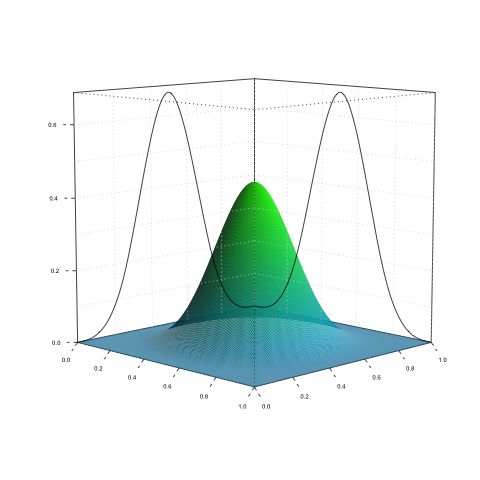
\includegraphics[width=4in, height=4in]{bicubic_basis_function.png}
 
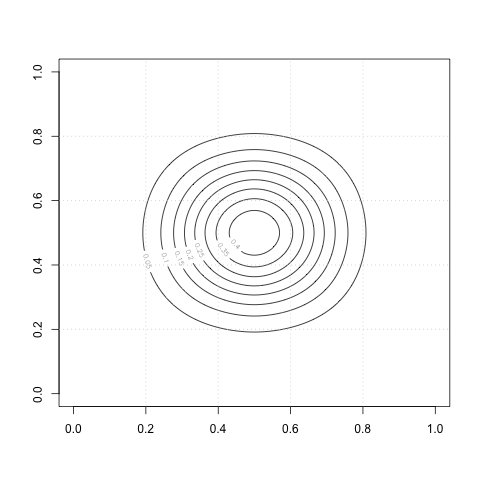
\includegraphics[width=4in, height=4in]{bicubic_bspline_contour.png}
\caption{Tensor product of two cubic B-splines}
\label{fig:bicubic_BS}
\end{figure}

\begin{figure}[H]
  \centering
  \graphicspath{{img/}}
  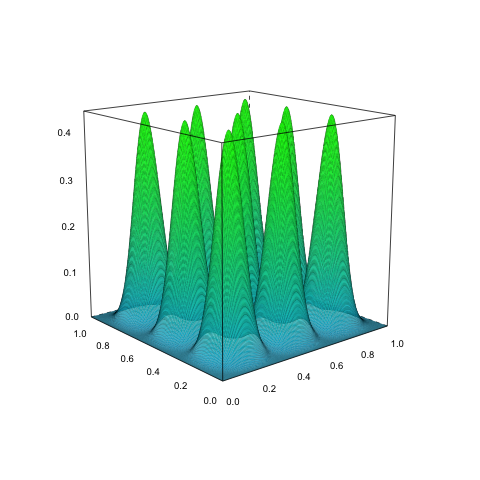
\includegraphics[width=5in,height=5in]{sparse_bicubic_basis.png}
  \caption{A subset of a full bivariate basis of cubic B-splines}\label{fig:sparse_bicubic_BS_basis}
\end{figure}

\subsection{Regularization with difference penalties} \label{subsection:univariate-psplines}

The minimizer of \ref{eq:loglikelihood} honors the fidelity to the data, so to balance the complexity of the fitted function with the goodness of fit to the data, we can append a penalty to the negative log likelihood to control the fitted function. By using rich B-spline bases for $l$ and $m$ alongside discrete difference penalties on the spline coefficients, we can achieve as much smoothness of the fitted function in both the $l$ and $m$ dimensions as desired. \cite{o1986statistical} was the first to propose using a rich B-spline basis and using a penalty to restrict the flexibility of the fitted curve, like \citet{wahba1990spline} applying a penalty to the second derivative of the fitted curve:
\[
J = \int_0^1 \left[ f^{\prime \prime}\left(l\right)\right]^2\;dx.
\]

For a B-spline of the form
\[
f\left(x\right) = \sum\limits_{j=1}^n \theta_i B_j\left(x\right),
\]
one can derive a banded matrix $P$ using the properties of B-splines such that 
 \[
 J = \theta^\prime P \theta
 \] 
 \noindent
 where $\theta = \left(\theta_1,\dots, \theta_n\right)$. The $i$-$j^{th}$ element of $P$ is given by
 \[
 p_{ij} = \int_0^1 B_i^{\prime \prime} \left( x \right)B_j^{\prime \prime} \left( x \right)\;dx.
 \]

%As discussed in Section 2, we can define an entire class of functional autoregressive models using only the $l$ direction, and additionally, as discussed in Section 3, there is a natural expectation about the functional form of the autoregressive coefficient function (and hence covariance) as a function of $l$. The use of smoothing splines to estimate $\phi$ outlined in Section~\ref{} yields smooth null models, but smoothness of the elements of the Cholesky factor alone may not lead to desirable structure in the inverse covariance matrix.  

%
%These approaches implicitly adopt different notions of sparsity. Like \citet{huang2006covariance} and \citet{levina2008sparse}, our aim is to regularize the inverse of the covariance matrix through the Cholesky factor. Expressing the varying coefficient function using a tensor product basis expansion builds the foundation for a flexible estimation framework within which employing multiple notions of smoothness is simple and straightforward. 
%

In some applications, it is useful to work with third and fourth order differences, since for large values of $\lambda$, the fitted curve approaches a parametric polynomial model. This may be of particular interest in the context of estimating the elements of the Cholesky factor, as many have proposed simple parametric functions of lag only for $\phi^*$, such as low order polynomials. See \citet{pourahmadi1999joint}. However, with the use of higher order derivatives, the computation of $P$ is nontrivial and becomes very tedious. \citet{eilers1996flexible} were the first to propose P-splines, or \emph{penalized B-splines}, as an approach to nonparametric regression. P-splines circumvent complexity associated with constructing such penalty matrices by omitting derivatives and integrals altogether, replacing them with finite differences and sums. 

Instead, flexibility of the fitted function is controlled by using a discrete penalty matrix based on finite difference formulas. Smoothness of the fitted function is achieved by first using a rich B-spline basis with equally spaced knots to purposefully overfit the smooth coefficient vectors; this eliminates the difficulty of choosing the optimal set of knots. Then by attaching a difference penalty to the goodness of fit measure, one may prevent overfitting and make a potentially ill-conditioned fitting procedure a well-conditioned one. The finite difference penalty is simple to compute and can be handled mechanically for any order of the differences. Since it is easily introduced into regression equations, it is feasible to evaluate the impact of different orders of the differences on the fitted model.  Using the properties of B-splines, it is straightforward to show that the difference penalty of order $d$ is a good discrete approximation to the integrated square of the $d^{th}$ derivative, so little is lost by replacing the derivative-based penalty with

\begin{equation} \label{eq:bspline-difference-penalty}
J_d\left( f \right) = \sum_{j=d}^n \left(\Delta^d \theta_j\right)^2
\end{equation} 
\noindent
where $\theta = \left( \theta_1,\dots,\theta_n \right)$. Let $D_d$ denote the matrix difference operator: $D_d\theta = \Delta^d \theta$, where

 \begin{align*}
 \Delta \theta_j &= \theta_j - \theta_{j-1}, \quad  \Delta^2 \theta_j = \Delta\left(\Delta \theta_j\right) = \theta_j - 2\theta_{j-1} + \theta_{j-2}
 \end{align*}
\noindent 
In general,
\begin{equation*}
\Delta^d \theta_j = \Delta\left(\Delta^{d-1} \theta_j \right).
\end{equation*} 
\noindent
Then, \ref{eq:bspline-difference-penalty} can be written in terms of the squared norm of the difference operator applied to the vector of B-spline coefficients:
\begin{align} 
\begin{split} \label{eq:bspline-difference-penalty-vector-form}
J_d\left( f \right) &= \vert \vert D_d\theta \vert \vert^2 \\
&= \theta^\prime P_d \theta
\end{split}
\end{align}
\noindent
where $P_d = D_d^\prime D_d$.  To examine the connection between the second-derivative penalty to the penalty on second-order differences of the B-spline coefficients, we only need to employ straightforward calculus and exploit the recursive property of the B-spline basis functions:

\begin{equation*} 
\int_0^1 \left[ f^{\prime \prime}\left(x\right)\right]^2\;dx = \int_{0}^{1} \left\{ \sum\limits_{j=1}^n  \theta_j B_{j,3}^{\prime \prime} \left(l\right) \right\}^2\; dl.
\end{equation*}
\noindent
The derivative properties of B-splines permits this to be written as 
\begin{equation*} \label{eq:second-derivative-bspline-penalty}
\int_0^1 \left[ f^{\prime \prime}\left(x\right)\right]^2\;dx =  \int_{0}^{1}  \bigg[ \sum\limits_{j=1}^n \sum\limits_{k=1}^n \Delta^2 \theta_j \Delta^2 \theta_k B_{j,1}\left(l\right)B_{k,1}\left(l\right)\bigg]\; dl  . 
\end{equation*}
\noindent
Most of the cross products of $B_{j,1}\left(x\right)$ and $B_{k,1}\left( x \right)$ vanish since B-splines of degree 1 only overlap when $j$ is $k-1$, $k$, or $k+1$. Thus, we have that
\begin{align}
\begin{split}
\int_0^1 \left[ f^{\prime \prime}\left(x\right)\right]^2\;dx  = {} &  \int_0^1 \bigg[ \left\{ \sum\limits_{j=1}^n   \Delta^2 \theta_j  B_j\left(l,1\right)  \right\}^2  + 2 \sum_{j}\Delta^2 \theta_j\Delta^2 \theta_{j-1}B_j\left(l,1\right)B_{j-1}\left(l,1\right) \bigg]\; dl \\ 
= {} & \sum \limits_{j=1}^n  \left( \Delta^2\theta_j \right)^2 \int_0^1 B_j^2\left(l,1\right)\;dl \\
   &{} \;\;\;\;\;\;\;\;\;\;\;\;\;\;\;\;\;\; + 2 \sum\limits_{j=1}^n \Delta^2 \theta_j\Delta^2 \theta_{j-1} \int_0^1 B_j\left(l,1\right)B_{j-1}\left(l,1\right)\;dl 
\end{split}
\end{align}
\noindent
which can be written as
\begin{equation} \label{eq:derivative-penalty-difference-penalty-connection}
\int_0^1 \left[ f^{\prime \prime}\left(x\right)\right]^2\;dx  = c_1 \sum\limits_{j=2}^n \left( \Delta^2 \theta_j\right)^2 + c_2 \sum\limits_{j=3}^n \Delta^2 \theta_j\Delta^2 \theta_{j-1}
\end{equation}
\noindent
Given a set of equidistant knots, the constants $c_1$ and $c_2$ are given by
\begin{equation}
\begin{split}
c_1 & =   \int_0^1 B_{j,1}^2\left(x\right) dx\\
c_2 & = \int_0^1 B_{j,1}\left(x\right)B_{j-1,1}\left(x\right) dx.
\end{split}
\end{equation}

This gives us that the traditional smoothness penalty on the squared second derivative can be written as a linear combination of a penalty on the second-order differences of the B-spline coefficients \ref{eq:bspline-difference-penalty} and the sum of the cross products of neighboring second differences. The second term in \ref{eq:derivative-penalty-difference-penalty-connection} leads to a complex objective function when minimizing the penalized likelihood, where seven adjacent spline coefficients occur, as opposed to five if only the first term in \ref{eq:derivative-penalty-difference-penalty-connection} is used in the penalty. The added complexity is a consequence of overlapping B-splines, which quickly increases when using higher order differences and higher order B-splines. We can seamlessly augment the likelihood with the difference penalty to achieve smooth fitted functions without the complexity posed by the derivative-based penalty.
%citet{chen2011efficient}, citet{pourahmadi1999joint}, and citet{pourahmadi2002dynamic} have elicited parametric models for the generalized autoregressive coefficients, letting the GARPs depend only on the distance between two time points.

A smoother sequence of coefficients leads to a smoother curve, as illustrated in Figure~\ref{fig:second_ord_PS_pen_SML_lambda}.  The relationship between P-spline curves and their coefficients is easily characterized if we consider the coefficients as the skeleton of the function, and draping the B-splines over them puts the flesh on the bones. As long as the coefficient sequence is smooth, the number of basis functions (and coefficients) is unimportant since the penalty ensures the smoothness of the skeleton and that the fitting procedure is well-conditioned. Figure~\ref{fig:overcomplete_basis_pspline} illustrates this utility of the penalty for simulated data; there are $m=10$ observations and $60$ cubic B-splines. This property of P-splines cannot be overly appreciated because it frees us from the concern of choosing the optimal set of knots. Unless computational constraints are of concern, which is possible with large models, it is prudent to use even more B-splines. Figure~\ref{fig:PS_penalty_section_figure_2} shows how the fitted function changes as the tuning parameter varies when the data are sparsely sampled. P-splines enjoy a number of additional advantageous properties, many of which are inherited from the attractive properties of B-splines. See \citet{eilers1996flexible}  for a detailed presentation. 

\begin{figure}[H] \label{fig:PS-smoothing-figure-1}
\begin{subfigure}{.5\textwidth}
  \centering
   \graphicspath{{img/}}
  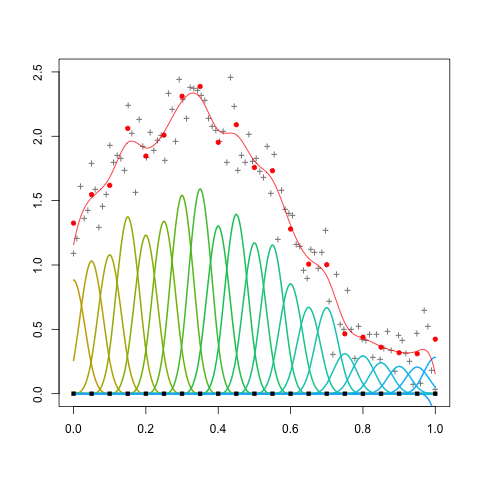
\includegraphics[scale=0.5]{pspline_pord2_xsmall_lambda.png}
  \label{fig:pspline_small_lambda}
\end{subfigure}
\begin{subfigure}{.5\textwidth}
  \centering
   \graphicspath{{img/}}
  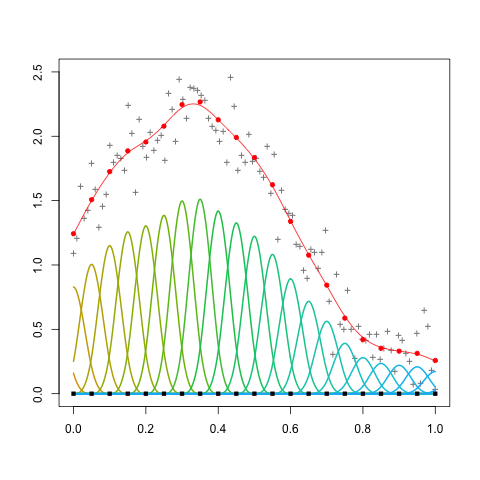
\includegraphics[scale=0.5]{pspline_pord2_small_lambda.png}
  \label{fig:pspline_small_lambda}
\end{subfigure}
\begin{subfigure}{.5\textwidth}
  \centering
   \graphicspath{{img/}}
  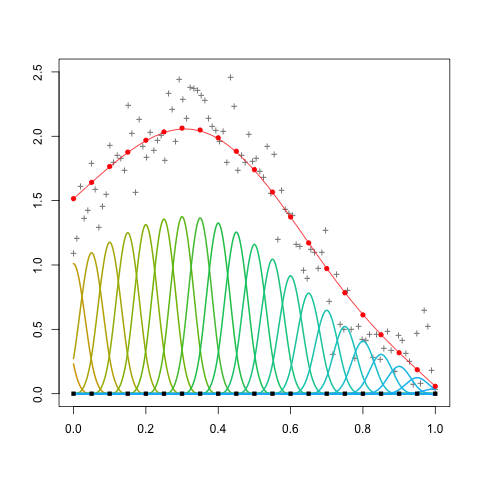
\includegraphics[scale=0.5]{pspline_pord2_medium_lambda.png}
  \label{fig:pspline_small_lambda}
\end{subfigure}
\begin{subfigure}{.5\textwidth}
  \centering
   \graphicspath{{img/}}
  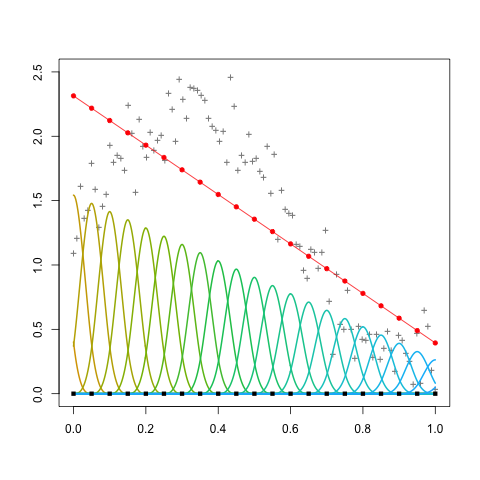
\includegraphics[scale=0.5]{pspline_pord2_large_lambda.png}
  \label{fig:pspline_small_lambda}
\end{subfigure}
\caption{\textit{Illustration of the impact of the second order difference penalty. The number of B-splines used is the same in each plot, with the value of the penalty parameter increasing from left to right and top to bottom across each plot. The fitted curve in the upper left plot is the most ``wiggly'' of any of the fits, as the penalty plays the weakest roll in the fitted coefficients there. The red circles are the values of each of the B-spline coefficients; as the penalty increases, they form as smoother sequence as we move across the four plots, which results in a smoother fitted function. As the penalty parameter approaches infinity, the fit approaches a linear function as shown in the bottom right plot.}}
\label{fig:second-ord-PS-pen-SML-lambda}
\end{figure}


%First, unlike many types of kernel smoothers, P-splines show no boundary effects i.e. the spreading of the fitted curve outside of the physical domain of the data, usually while also bending toward zero. See \citet{eilers1996flexible} Section 8 for a detailed discussion.

%P-splines can fit polynomial data exactly. Given data $\left(l_i,y_i\right)$, if the $y_i$ are a polynomial in $l$ of degree $k$, then B-splines of degree $k$ or higher will fit the data exactly.  The same is true for P-splines if the order of the penalty is $k+1$ or higher, irrespective of the value of $\lambda$. An informal proof is left to the appendix.
%
%Under a difference penalty of order $k$, the fitted function will approach a polynomial of degree $k-1$ for large values of $\lambda$ as long as the degree of the B-splines is greater than or equal to $k$. This can be shown by once again considering the relationship between the derivatives of a B-spline fit and the differences in neighboring coefficients; detailed discussion is left to the appendix. Figure~\ref{fig:PS_penalty_section_figure_6} visually demonstrates this property by examining the behavior of the fitted function as the tuning parameter varies under a difference penalty of order $d=0,1,2,3$.
%
%We will leverage several properties of the smoothing matrix, $H$, for model evaluation and selection, so focus on the linearized smoothing problem solved at each value of the penalty parameter, $\lambda$, is prudent. The trace of $H$ approaches the order of the differencing operator, $k$ for larges values of $\lambda$. The trace of the smoothing matrix is a useful measure of effective model dimension, so understanding its limiting behavior is important. 



To extend these results to the bivariate setting for regularizing of $\phi^*$, the only modification to the differencing procedure in one dimension necessary is the addition of a second difference penalty, one for each variable $l$ and $m$. We append the pair of penalties to the negative log likelihood \ref{eq:loglikelihood} and take the estimator of $\phi^*$ to correspond to the B-spline coefficients minimizing

\begin{align} 
\begin{split}\label{eq:unfolded-difference-penalty-log-likelihood}
-2L + J\left(\phi^*\right) = \sum_{i=1}^N \sum_{j=2}^{m_i} \sigma\left({t_j}\right)^{-2} \left\{y_{ij} - \sum_{k=1}^{j-1} \left( \sum_{r=1}^L \sum_{s=1}^K \theta_{rs} B_r\left(l_{ijk}\right)B_s\left(m_{ijk}\right)\right)y_{ik} \right\}^2 \\ 
+ \lambda_l \sum_{r^\prime=1}^K \vert D_{d_{\ms l}} \theta_{r^\prime \cdot} \vert^2 + \lambda_m \sum_{s^\prime=1}^L \vert D_{d_{\ms m}} \theta_{\cdot s^\prime} \vert^2.
\end{split}
\end{align}


%\begin{align*}\label{eq:unfolded-row-column-difference-penalty}
%\mathcal{Q}=\sum_{i=1}^n \sum_{j=2}^{m_i} \sigma_{ij}^{-2} \left[y_{ij} - \sum_{k=1}^{j-1}\left(\sum_{i=1}^K \sum_{j=1}^L \theta_{ij} B_{i}\left(l_{ijk}\right) B_{j}\left( m_{ijk} \right)  \right) y_{ik} \right]^2 \\
%\mbox{\;\;\;\;\;\;\;\;}+ \lambda_l \sum_{k} \vert D_d \theta_{k \cdot} \vert^2 + \lambda_m \sum_{l} \vert D_{\ms d_{\ms m}} \theta_{\cdot l} \vert^2 
%\end{align*}

\noindent
where $\theta_{k \cdot}$ and $\theta_{\cdot l}$ denote the $k^{th}$ row and $l^{th}$ column of $\Theta$, respectively. The first term in\ref{eq:unfolded-row-column-difference-penalty} imposes a difference penalty of order $d_{\ms l}$ on the rows of the coefficient matrix while the second term places a difference penalty (of possible different order $d_{\ms m}$) on the columns. We give each direction its own smoothing parameter to permit anisotropic smoothing; however, one could opt to use a single smoothing parameter for both directions and dodge the added work of optimizing the amount of smoothing with two separate parameters. Figure ~\ref{fig:2d_PS_penalty_demo} shows a potential result of heavy column penalization (left) and heavy row penalization (right) under a second order difference penalty on each row and each column for large values of $\lambda_l$ and $\lambda_m$. The figure demonstrates that the limiting behaviour of each row and column is linear, but the resulting surface may exhibit slope reversals from one row (column) to the next. 


\begin{figure}[H] \label{fig:2d_PS_penalty_demo}
 \begin{subfigure}{.48\textwidth}
  \centering
   \graphicspath{{img/}}
 \includegraphics[scale=0.5]{"model selection/effective dimension/2d_PS_section_figure1_big_col_lambda"}
 \caption{\textit{heavy column penalty}}
 \label{fig:2D_PS_big_col_penalty}
 \end{subfigure}
 \begin{subfigure}{.48\textwidth}
  \centering
   \graphicspath{{img/}}
  \includegraphics[scale=0.5]{"model selection/effective dimension/2d_PS_section_figure1_big_row_lambda"}
 \caption{\textit{heavy row penalty}}
\label{fig:2D_PS_big_row_penalty}
 \end{subfigure}
 \caption{\textit{Nine cubic B-spline tensor products with heavy linear column penalty and heavy linear row penalty}}
\end{figure}
\noindent
We take the estimator of $\phi^*$ to be the minimizer of 
It is computationally advantageous to express the coefficient matrix in ``unfolded'' notation, which allows us to express the varying coefficient function at the observed coordinate grid as in the usual multiple regression form:

\begin{equation*}
\mbox{vec}\left\{\phi^*\left(l,m\right)\right\} = B \theta
\end{equation*}
\noindent
Stacking the columns of $\Theta$ gives the vectorized coefficient matrix $\theta = \mbox{vec}\left( \Theta \right)$. The $p \times KL$ tensor product basis $B$ is constructed from the tensor product of the marginal B-spline bases defined in \citet{eilers2006fast} as the \textit{row-wise Kronecker product} of the individual bases:

\begin{equation} \label{eq:rowwise-kronecker-product}
B = B_l \square B_m = \left( B_m \otimes 1^\prime_{K} \right) \odot \left(1^\prime_{L} \otimes  B_l  \right).
\end{equation}
\noindent
The operator $\odot$ denotes the element-wise matrix product; $1_K$ ($1_L$) denotes the column vector of ones having length $K$ ($L$.) The operations in \ref{eq:rowwise-kronecker-product} construct $B$ such that the $i^{th}$ row of $B_m\square B_l$ is the Kronecker product of the corresponding rows of $B_m$ and $B_l$. The penalty in \ref{eq:unfolded-row-column-difference-penalty} can also be compactly expressed:

\begin{equation*} \label{eq:tensor-product-penalty}
\lambda_l \vert \vert P_l \theta \vert \vert^2 + \lambda_m \vert \vert P_m \theta \vert\vert^2
\end{equation*}

where $P_l = I_L \otimes D_{d_{\ms l}}^\prime D_{d_{\ms l}} $ and $P_m =  D_{d_{\ms m}}^\prime D_{d_{\ms m}} \otimes I_K$. We define the matrix $W$ of historical regressors so that \ref{eq:unfolded-difference-penalty-log-likelihood} can be written in matrix form as

\begin{equation} \label{eq:tensor-pspline-objective-function}
-2L + J\left(\phi^*\right) = \left( Y - WB\theta\right)^\prime D^{-1}\left( Y - WB\theta\right)  + \lambda_l \vert\vert P_l \theta \vert\vert^2 + \lambda_m \vert\vert P_m \theta\vert \vert^2,
\end{equation}
\noindent
with $\hat{\theta}$ solving the system of equations 
\begin{equation} \label{eq:tensor-pspline-normal-equations}
\left[ \left(WB\right)^\prime D^{-1} WB +  \lambda_l P_l+ \lambda_m P_m\right]\theta = \left(W B\right)^\prime D^{-1}Y
\end{equation}
\noindent
From \ref{eq:tensor-pspline-normal-equations}, we note that the system of equations depends on basis coefficients remains fixed at $KL$, even as the number of observations increases.   The grid of regression coefficients can be recovered by arranging the elements of $\hat{\theta}$ into a matrix of $L$ columns having length $K$. 


\section{Model selection and tuning parameter estimation}

\subsection{The limiting behaviour of $H_\lambda$}


The inspection of the hat matrix 

\[
H_\lambda = W B\left(W B^\prime W B +  \lambda_l P_l + \lambda_m P_m \right)^{-1} \left(W B\right)^\prime D^{-1}.
\]
\noindent
and its properties are integral for assessing model complexity and selecting the optimal values of the tuning parameters $\lambda_l$ and $\lambda_m.$  Summarizing the complexity of a fitted P-spline is far from a trivial task; one must simultaneously consider the value of the smoothing parameter, the number of basis functions in the B-spline basis, as well as the order of the difference penalties. We follow \cite{eilers1996flexible} and\cite{marx2005multidimensional} assess model complexity as discussed in cite{hastie1990generalized}, who proposed to use the trace of the smoother matrix as an approximation  to the effective dimensions of linear smoother. The \emph{effective dimension} is easily obtained and combines the effect of all three of these elements: 

%This approach to approximating the effective model dimension is also consistent with \cite{ye1998measuring}, who constructed a generalization of the concept of a model's degrees of freedom using the idea that the degrees of freedom can also be interpreted as the sum of the sensitivity of each fitted value with respect to the corresponding observed value.  For smoothing matrix $H$, the predicted response values are given by $\hat{y} = H y$. Writing
%
%\begin{align*}
%\frac{\partial \hat{y_i}}{\partial y_i} = \frac{\partial }{\partial y_i} \sum_{j} h_{ij} y_j = h_{ii},
%\end{align*}
%\noindent
%we see that the latter interpretation of the effective model dimension reduces to calculating the trace of the hat matrix. Thus we take the effective dimension to be 
%\begin{align}
%\textup{ED}\left(\lambda\right) &= \textup{tr}\left(H\right) \nonumber \\
%&= \textup{tr}\bigg[ B\left( B^T B + \lambda D^T D \right)^{-1} B^T\bigg], \label{eq:hat_matrix_trace}
%\end{align}

\begin{align}
\begin{split} \label{eq:hat-matrix-trace}
\textup{ED} &= \textup{tr} \left[ H_\lambda \right]\\
&= \textup{tr}\bigg[\left[WB \left(WB\right)^\prime D^{-1}WB +  \lambda_l P_l+ \lambda_m P_m\right]^{-1} \left(W B\right)^\prime D^{-1}  \bigg]
\end{split}
\end{align}
\noindent
When the number of basis functions is significantly smaller than the sample size, it is computationally advantageous to use the cyclic property of the trace: 

\begin{equation*}
\textup{tr}\bigg[\left[ \left(WB\right)^\prime D^{-1}WB +  \lambda_l P_l+ \lambda_m P_m\right]^{-1} \left(W B\right)^\prime D^{-1} WB  \bigg],
\end{equation*}
\noindent
which requires computing the trace of a $KL \times KL$ matrix. The effective dimension approaches $d_l + d_m$, the order of the differencing operator, as $\lambda$ increases, where $d_l$ and $d_m$ denote the orders of the difference penalties in the $l$ and $m$ directions, respectively.  Let
\begin{equation*}
Q = \left(W B\right)^\prime D^{-1} WB \qquad \mbox{and} \qquad Q_\lambda = P.
\end{equation*}
Using properties of the matrix trace, we can write
\begin{align*}
%\begin{split}
\mbox{tr}\left(H_\lambda \right) &= \mbox{tr}\bigg[ \left(Q + Q_\lambda \right)^{-1}Q \bigg]\\
&=\mbox{tr}\bigg[ Q^{1/2}\left(Q + Q_\lambda \right)^{-1}Q^{1/2} \bigg] \\
&=\mbox{tr}\bigg[\left(I + Q^{-{1/2}}Q_\lambda Q^{-{1/2}} \right)^{-1} \bigg]
%\end{split}
\end{align*}
Define $L \equiv Q^{-{1/2}}Q_\lambda Q^{-{1/2}}$. Then
\begin{equation*}
\mbox{tr}\left(H_\lambda \right) = \mbox{tr}\bigg[\left(I + \lambda L \right)^{-1} \bigg] = \sum_{j=1}^n \frac{1}{1 + \lambda \gamma_j}
\end{equation*}
 where $\gamma_j$, $j=1,\dots,n$ are the eigenvalues of $L$. $Q_\lambda$ has exactly $d_l + d_m$ eigenvalues equal to zero. Hence, $L$ has $d_l + d_m$ zero eigenvalues. For large $\lambda$, only the $d_l + d_m$ terms with $\gamma_j=0$ contribute to the sum which gives the trace of $H$, so that
 \[
\lim_{\lambda \rightarrow \infty  } \mbox{tr}\left(H\right) = d_l + d_m.
 \]
%
%A further simplification of \ref{eq:hat-matrix-trace}
%
%\begin{align*} 
%\left(B^T B + \lambda D^T D \right)^{-1} B^T B &= \left(B^T B + \lambda D^T D \right)^{-1} \left( B^T B + \lambda D^T D - \lambda D^T D\right) \nonumber \\
%&= I - \lambda\left(B^T B + \lambda D^T D \right)^{-1} D^T D \label{eq:cyclic_hat_matrix_simplification}
%\end{align*}
%
%\begin{align*} 
%\left[\left(WB\right)^\prime D^{-1}WB +  \lambda_l P_l+ \lambda_m P_m\right]^{-1} \left(W B \right)^\prime D^{-1} WB  &= \left[\left(WB\right)^\prime D^{-1}WB +  \lambda_l P_l+ \lambda_m P_m\right]^{-1}\left(W B \right)^\prime D^{-1} \times \\
%&\mbox{\;\;\;\;\;\;\;\;\;\;\;\;\;\;\;\;\;\;\;\;\;} \left[WB + \lambda_l P_l+ \lambda_m P_m - \left(\lambda_l P_l+ \lambda_m P_m\right) \right] \\
%&= I - \lambda\left(B^T B + \lambda D^T D \right)^{-1} D^T D \label{eq:cyclic_hat_matrix_simplification}
%\end{align*}
%
%
%
%Equation~\ref{eq:cyclic_hat_matrix_simplification} cleanly shows that the effective dimension is always less than $n$, the number of B-spline used in the regression basis; further, the effective dimension is always smaller than $\min\left(m,n\right)$. A formal proof follows below. This is illustrated in 

Figure~\ref{fig:PS_ED_figure_1} shows how the effective dimension on a univariate P-spline changes with the smoothing parameter for the ten simulated observations in Figure~\ref{fig:overcomplete_basis_pspline} using 60 B-spline basis functions. For small $\lambda$, the effective dimension approaches $m$. As $\lambda$ increases, the effective dimension approaches the order of the difference penalty, $d$. It is worth pointing out here that there are no problems incurred when smoothing with many more B-splines than observations since the effective model dimension is always less than $m$, for all $\lambda$. 


\begin{figure}[H]
\begin{subfigure}{.5\textwidth}
  \centering
   \graphicspath{{img/}}
  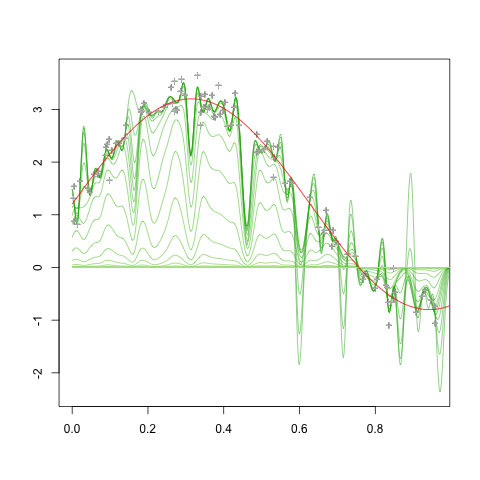
\includegraphics[scale=0.5]{PS_penalty_section_figure_6_order_0.png}
  %\label{fig:pspline_small_lambda}
\caption{$d=0$ }
\end{subfigure}
\begin{subfigure}{.5\textwidth}
  \centering
   \graphicspath{{img/}}
  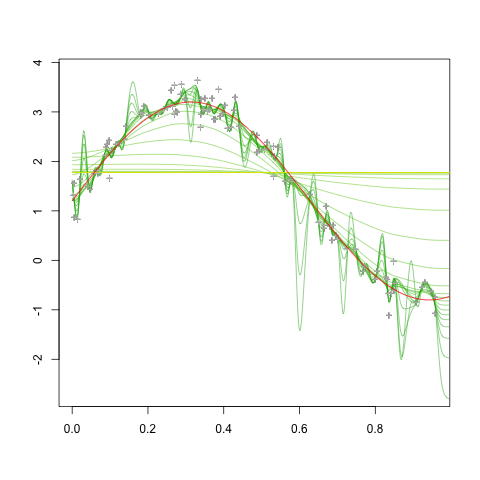
\includegraphics[scale=0.5]{PS_penalty_section_figure_6_order_1.png}
 % \label{fig:pspline_small_lambda}
\caption{$d=1$}
\end{subfigure}
\begin{subfigure}{.5\textwidth}
  \centering
   \graphicspath{{img/}}
  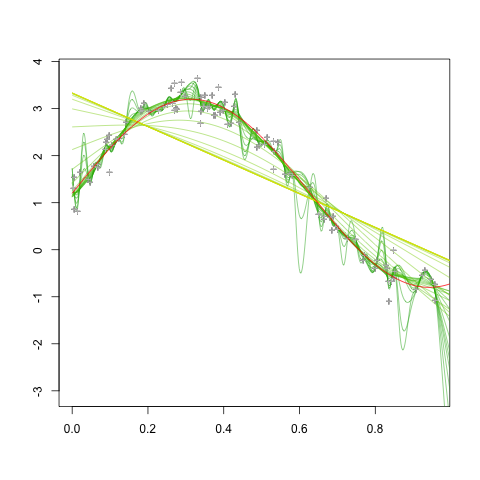
\includegraphics[scale=0.5]{PS_penalty_section_figure_6_order_2.png}
  %\label{fig:pspline_small_lambda}
\caption{$d=2$}
\end{subfigure}
\begin{subfigure}{.5\textwidth}
  \centering
   \graphicspath{{img/}}
  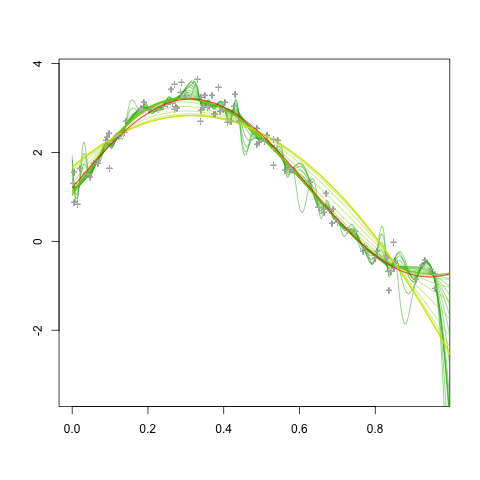
\includegraphics[scale=0.5]{PS_penalty_section_figure_6_order_3.png}
  %\label{fig:pspline_small_lambda}
\caption{$d=3$}
\end{subfigure}
\caption{\textit{Illustration of the impact of the order of the difference penalty. The number of B-splines used is the same in each plot, with the penalty parameter varying from across the same grid of values. The fitted curves in the upper left plot correspond to the difference penalty of order $0$, where $\vert D_0 \alpha \vert^2 = \sum_{i=1}^n \alpha_i^2$, analogous to ridge regression using the B-spline basis as regression covariates. The fitted curves approach polynomials of degree $d-1$ as $\lambda \rightarrow \infty$, as discussed in \ref{eq:PS_properties} \ref{eq:PS_property_3}.}}
\label{fig:PS_penalty_section_figure_6}
\end{figure}

%%====================================================================================
%%====================================================================================


%Cross validation prediction error is a well-known measure of the predictive power of a P-spline model for given values of the smoothing parameters $\lambda_l$, $\lambda_m$ . 
Cross validation and its variants have long been utilized for smoothing parameter selection in spline models, and their properties have been studied extensively. A short list of supplemental references include \cite{craven1978smoothing}, \cite{wahba1985comparison}, \cite{hardle1988far}, \cite{hardle1992applied}, and \cite{wahba1990spline}. There are a number of ways to calculate a measure of cross validated prediction error; we first focus on the leave-one-out method. Let $\hat{y}_{-i}$ denote the predicted value for the observation $y_i$ when $y_i$ itself is removed from the data we use to fit the model. We can calculate these predictions for each observation in the data set to obtain the prediction error:

\begin{equation} \label{eq:LOOCV_def}
\textup{CV}\left(\lambda\right) = \frac{1}{m}\sum_{i=1}^m \left(  y_i - \hat{y}_{-i}\right)^2, 
\end{equation}
Brute force calculation of \ref{eq:LOOCV_def} is generally impractical, especially if the number of observations is large. However, this labor can be sidestepped using the following fact: 

\begin{equation*}
\hat{y} = Hy = B\left(B^TB + \lambda D_d^T D_d \right)^{-1} B^T y
\end{equation*}

One can show that 

\begin{equation} \label{eq:LOO_residual}
y_i - \hat{y}_{-i} = \left(y_i - \hat{y}_{i}\right)/\left(1-h_{ii}\right),
\end{equation}
\noindent
and the diagonal elements of $H$ can be calculated quickly. An informal proof of \label{eq:LOO_residual} is as follows: suppose that we change the $i^{th}$ element of $y$, obtaining a new response vector $y^*$. Then $\hat{y}^* = H y^*$.

 Since 
 \[
 \hat{y}_i = \sum_{j} h_{ij} y_j \qquad \textup{and} \qquad \hat{y}_{-i} = \sum_{j} h_{ij} y_j^*,
 \]
 \noindent
 then
 \[
 \hat{y}_i - \hat{y}_{-i} = \sum_j h_{ij} \left(y_i - y_i^*\right) = h_{ii} \left(y_i - y_i^*\right).  
\]


For generalized cross-validation \cite{wahba1990spline}, we compute 
\begin{equation} \label{eq:GCV_def}
\textup{GCV}\left(\lambda\right) = \sum_{i=1}^m \frac{\left(  y_i - \hat{y}_i \right)^2}{\left(m-\sum_{j=1}^m h_{jj}\right)^2} 
\end{equation}

The difference between both quantities is generally small; the best $\lambda$ is the value that minimizes $\textup{CV}\left(\lambda\right)$ or $\textup{GCV}\left(\lambda\right)$. 
The smoothing matrix $H$ plays an integral role of calculating all of the model selection criteria we will discuss; within the context of both AIC and cross validation, the diagonal elements of $H$, $h_{ii}$ are of particular importance. Closely related to the problem of model selection is the ability to quantify model complexity. In classical regression theory, the degrees of freedom are clearly defined as the number of variables included in the model. \cite{eilers1996flexible} and\cite{marx2005multidimensional} refer to this measure of model complexity as the model's \emph{effective dimension} ED; they follow \cite{hastie1990generalized}, who discuss the effective dimensions of linear smoother and propose to use the trace of the smoother matrix as an approximation.

This approach to approximating the effective model dimension is also consistent with \cite{ye1998measuring}, who constructed a generalization of the concept of a model's degrees of freedom using the idea that the degrees of freedom can also be interpreted as the sum of the sensitivity of each fitted value with respect to the corresponding observed value.  For smoothing matrix $H$, the predicted response values are given by $\hat{y} = H y$. Writing

\begin{align*}
\frac{\partial \hat{y_i}}{\partial y_i} = \frac{\partial }{\partial y_i} \sum_{j} h_{ij} y_j = h_{ii},
\end{align*}
\noindent
we see that the latter interpretation of the effective model dimension reduces to calculating the trace of the hat matrix. Thus we take the effective dimension to be 
\begin{align}
\textup{ED}\left(\lambda\right) &= \textup{tr}\left(H\right) \nonumber \\
&= \textup{tr}\bigg[ B\left( B^T B + \lambda D^T D \right)^{-1} B^T\bigg], \label{eq:hat_matrix_trace}
\end{align}


{
\needsparaphrased{
[ INSERT PROOF HERE.]
}
}

An alternative approach to model selection is to minimize the information criterion (IC):
\[
\textup{IC}\left(\lambda\right) = -2\mathscr{l}\left(y, \hat{\beta}_\lambda \right) + c\; \textup{dim}\left(\hat{\beta}_\lambda\right)
\]

Special cases are when $c=2$, yielding the Akaike information criterion (AIC) and when $c=\log\left(m\right)$, yielding the Bayesian information criterion (BIC). The IC assesses the quality of a model by adjusting the log likelihood of the data under the fitted model to account for some measure of model complexity. In the classical linear model setting, the degrees of freedom serves as the measure of model complexity, is used for obtaining an unbiased estimate of the error variance, and thus, is necessary for comparing the performance of different models. In the case of the normal likelihood, AIC becomes

\begin{equation} \label{eq:univariate_AIC}
\textup{AIC}\left(\lambda\right) = %\sum_{i=1}^m \frac{\left( y_i - \hat{\mu}_i \right)^2}{\sigma^2} + 2\tr\left(H\right) - 2m\log\left(\sigma\right) - m\log 2\pi
\end{equation}

One may use CV to select the optimal value of $\lambda$, and then using the corresponding residuals gives a natural choice to use as an estimate of $\sigma^2$ for the computation of $\textup{AIC}\left(\lambda\right)$. It is practical to work with modified versions of $\textup{CV}\left(\lambda\right)$ and $\textup{GCV}\left(\lambda\right)$, with values that can be interpreted as estimates of the cross-validation standard deviation:

\begin{equation}
\begin{split}
\bar{\textup{CV}}\left(\lambda\right) &= \sqrt{\textup{CV}\left(\lambda\right)} \\
\bar{\textup{GCV}}\left(\lambda\right) &= \sqrt{m\textup{GCV}\left(\lambda\right)} \\
\end{split}
\end{equation}

Alternatively, one might note that an (approximately) unbiased estimate of the error variance is given by the sum of squared residuals divided by the error degrees of freedom, $m-\textup{ED}$.






% 
%\section{\emph{Approximate $\phi_1$, $\phi_2$, $\phi_{12}$ with B-splines.}}
%
%\begin{align}  
%\begin{split}\label{eq:l-m-marginal-basis}
%\phi^*\left(l,m \right) &= B \theta \\
%&= \phi_1\left(l\right)  + \phi_2\left(m\right)  + \phi_{12}\left(l,m\right)  \\
%&= \sum_{c=1}^{c_l} B_{\ms c}\left(l\right) \theta_{lc }  B_{\ms l} \theta_l + \sum_{c^\prime=1}^{c_m} B_{\ms{c^\prime}}  \left(  m \right)  \theta_{\ms{mc^\prime }}  \\
%&\mbox{\;\;\;\;\;\;\;\;\;\;\;\;\;\;\;\;\;\;\;\;\;\;\;\;\;\;\;\;\;\;} + \sum_{c=1}^{c_l} \sum_{{c^\prime}=1}^{c_m} B_{\ms c}\left(l\right) B_{\ms{c^\prime } }\left(m\right)\theta_{\ms{c c^\prime} } 
%\end{split}
%\end{align}
%
%where $\theta \equiv \left(\mu, \theta_{\ms{l}},\theta_{\ms{m}},\theta_{\ms{lm}}\right)^\prime $ and
%\begin{align*}
%B &\equiv \left[\; 1_p \; \vert \;  B_l  \; \vert \;   B_m \; \vert B_{\ms{lm}} \; \right] \\
%&= \left[\; 1_p \; \vert \;  B_l  \; \vert \;   B_m \; \vert  B_m \; \square \; B_l \right] 
%\end{align*}
%
% 

%
% 
%\section{\emph{PS-ANOVA model basis}}
%
%In matrix notation, Model \ref{eq:expanded-ps-anova-vc-model} becomes
%
%\begin{equation*}  
%E \left[ Y | W \right] = WB \theta,
%\end{equation*}
%\noindent
%where $W$ is the matrix of covariates holding the past values of $Y$, and $B$ is the $B$-spline regression basis:
%\begin{equation} \label{eq:SANOVA-basis-matrix}
%B = \left[\; 1_p \; \vert \;  B_l  \; \vert \;   B_m \; \vert B_{lm} \; \right]
%\end{equation}
%\noindent
%where 
%\begin{align*} \label{eq:rowwise-kronecker-product}
%B_{lm} &= B_m \; \square \; B_l \\
%&\equiv \left( B_m \otimes 1^\prime_{c_l} \right) \odot \left(1^\prime_{c_m} \otimes  B_l  \right).
%\end{align*}
% 
%
%



%%%%%%%%%%%%%%%%%%%%%%%%%%%%%%%%%


 
\section{\emph{Simulations: }$\Sigma = 0.3^2 I$\\
$N = 30$, $M=20$, $d_l = d_m= 0$}


    \begin{center}
    \begin{figure}[H]
    \graphicspath{{img/}}
 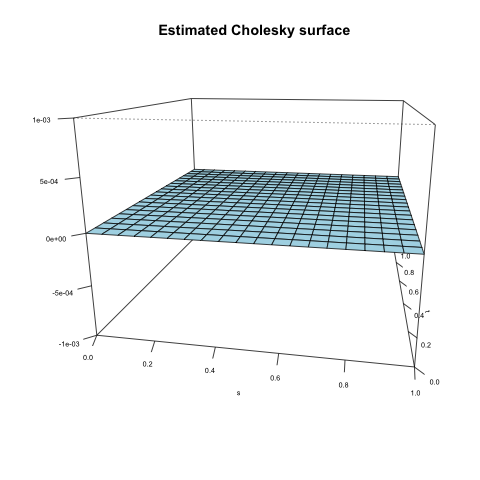
\includegraphics[width=5cm]{identity-cov-estimated-cholesky}
 \caption{Estimated $T$ }
 \end{figure}
     \end{center}
  

 


 
\section{\emph{Simulations: }$\Sigma = 0.3^2 I$\\
$N = 30$, $M=20$, $d_l = d_m= 0$}

\begin{center}
\begin{figure}[H] \label{row-col-differencing}
 \begin{subfigure}{.48\textwidth}
 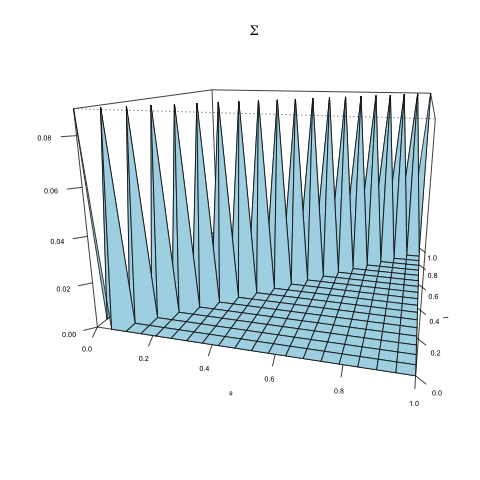
\includegraphics[width=4cm]{img/identity-cov-true-covariance}
 \caption{True $\Sigma$ }
 \end{subfigure}
 \begin{subfigure}{.48\textwidth}
  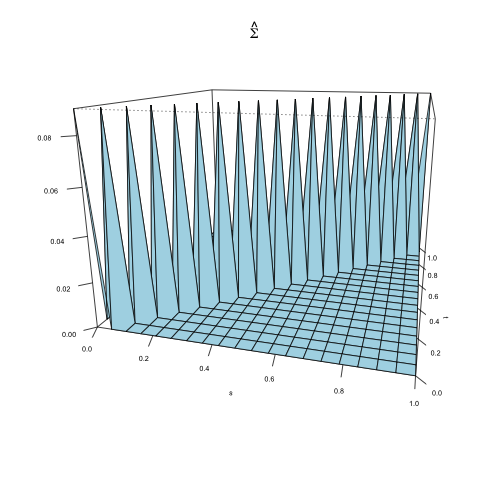
\includegraphics[width=4cm]{img/identity-cov-estimated-covariance}
 \caption{$\hat{\Omega}^{-1}$}
 \end{subfigure}
 \end{figure}
     \end{center}


 

%%%%%%%%%%%%%%%%%%%%%%%%%%%%%%%%%

 
\section{\emph{Simulations: }$\phi\left(s,t\right) = s-\frac{1}{2}$, $\sigma^2 = 0.3^2$\\
$N = 30$, $M=20$, $d_l = d_m= 2$}

\begin{center}
\begin{figure}[H]
 \begin{subfigure}{.48\textwidth}
 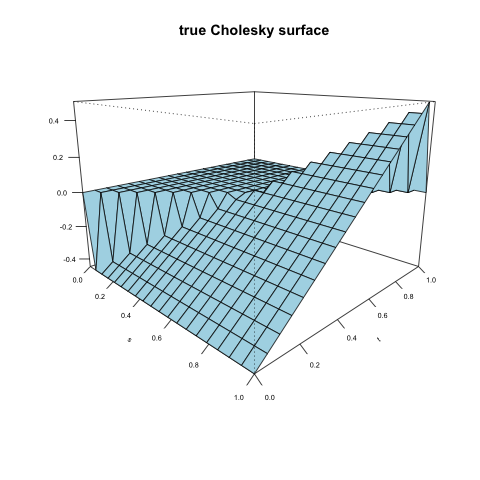
\includegraphics{img/linear-vc-model-true-cholesky}
 \caption{True $T$ }
 \end{subfigure}
     \begin{subfigure}{.48\textwidth}
 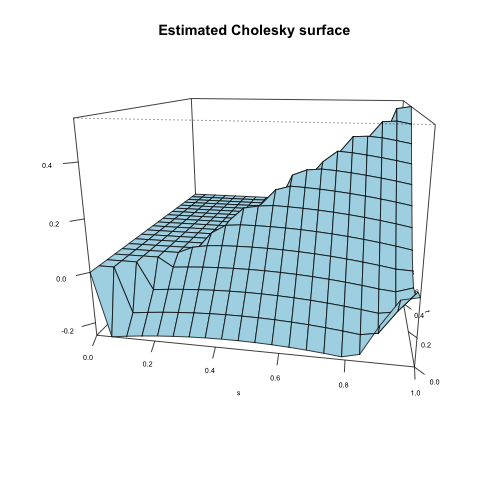
\includegraphics{img/linear-vc-model-estimated-cholesky}
 \caption{Estimated $T$}
 \end{subfigure}
     \end{figure}
\end{center}


 



 
\section{\emph{Simulations: }$\phi\left(s,t\right) = s-\frac{1}{2}$, $\sigma^2 = 0.3^2$\\
$N = 30$, $M=20$, $d_l = d_m= 2$}

 \begin{center}
\begin{figure}[H]
 \begin{subfigure}{.48\textwidth}
 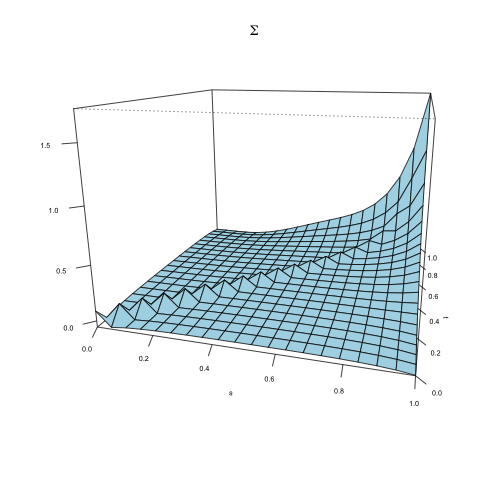
\includegraphics{img/linear-vc-model-true-covariance}
 \caption{$\Sigma$ }
 \end{subfigure}
 \begin{subfigure}{.48\textwidth}
 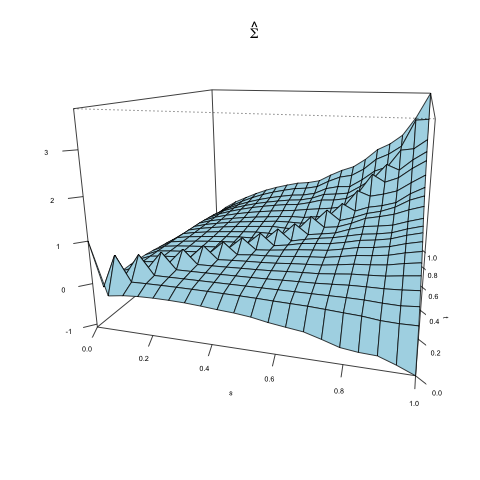
\includegraphics{img/linear-vc-model-estimated-covariance}
 \caption{$\hat{\Omega}^{-1}$}
 \end{subfigure}
 \end{figure}
     \end{center}


 
%%%%%%%%%%%%%%%%%%%%%%%%%%%%%%%%%



 
\section{\emph{Simulations: }$\Sigma = 0.7J + 0.3I$\\
$N = 30$, $M=20$, $d_l = 2$, $d_m= 1$}

  \begin{center}
\begin{figure}[H]
 \begin{subfigure}{.48\textwidth}
 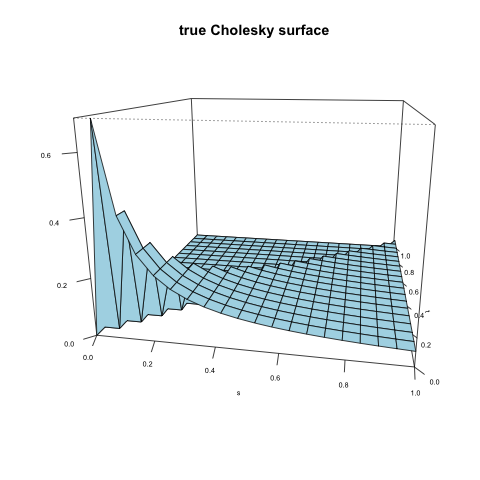
\includegraphics{img/compound-symmetry-true-cholesky}
 \caption{True $T$ }
 \end{subfigure}
 \begin{subfigure}{.48\textwidth}
  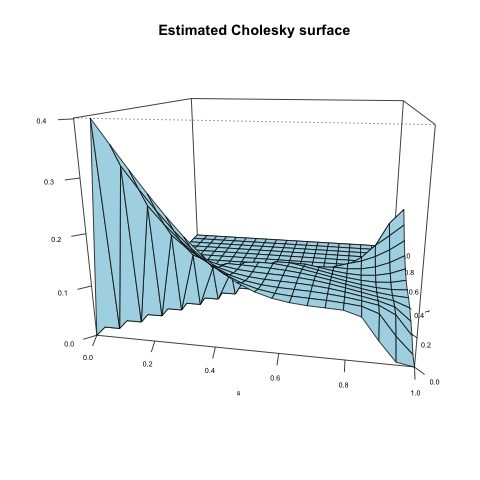
\includegraphics{img/compound-symmetry-estimated-cholesky}
 \caption{Estimated $T$}
 \end{subfigure}
\end{figure}
\end{center}


 



 
\section{\emph{Simulations: }$\Sigma = 0.7J + 0.3I$\\
$N = 30$, $M=20$, $d_l = 2$, $d_m= 1$}


  \begin{center}
\begin{figure}[H]
 \begin{subfigure}{.48\textwidth}
 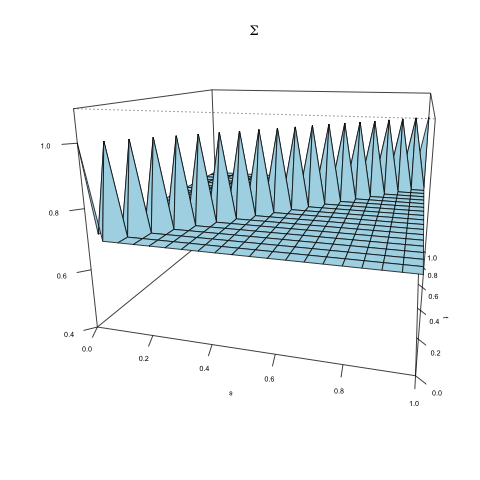
\includegraphics{img/compound-symmetry-true-covariance}
 \caption{$\Sigma$ }
 \end{subfigure}
  
 \begin{subfigure}{.48\textwidth}
 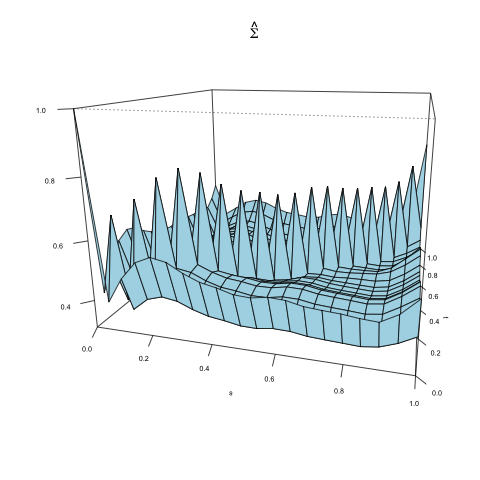
\includegraphics{img/compound-symmetry-estimated-covariance}
 \caption{$\hat{\Omega}^{-1}$}
 \end{subfigure}
 \end{figure}
     \end{center}



 
\section{\emph{Recruit the difference penalty to regulate.}}

For $f\left(x\right)=\sum \limits_{i=1}^{p} B_{i}\left(x\right) \theta_{i}$, approximate

\begin{align*}
%\begin{split}
\int_0^1 \left(f^{\prime \prime}\left(x\right)\right)^{\ms 2} \;dx &= \int_0^1 \bigg\{ \sum \limits_{i=1}^{p} B^{\prime \prime}_{i}\left(x\right) \theta_{i} \bigg\}^{\ms 2} \;dx \\ 
&= k_1 \sum_i \left( \Delta^{\ms 2} \theta_i \right)^{\ms 2} + k_2, 
%\end{split}
\end{align*}
\noindent
by
\[
\vert \vert D_{\ms 2} \theta \vert \vert^{\ms 2}, \qquad  D_{\ms 2} \theta= \left( \Delta^{\ms 2}\theta_{\ms 1},\dots,\Delta^{\ms 2}\theta_{\ms{p-2}} \right)^\prime 
\]
In general, 
\framebox{approximate $\int \limits_{\ms 0}^{\ms 1} \big(f^{\ms{\left(d\right)}}\big)^{\ms 2}\;dx$ with $\vert \vert D_{\ms d} \theta \vert \vert^{\ms 2} $ }
 


 
\section{\emph{Append the difference penalties to the log likelihood:}}

Find $\theta$ minimizing

\begin{align*}\label{eq:unfolded-row-column-difference-penalty}
\mathcal{Q}=\sum_{i=1}^n \sum_{j=2}^{m_i} \sigma_{ij}^{-2} \left[y_{ij} - \sum_{k=1}^{j-1}\left(\sum_{i=1}^K \sum_{j=1}^L \theta_{ij} B_{i}\left(l_{ijk}\right) B_{j}\left( m_{ijk} \right)  \right) y_{ik} \right]^2 \\
\mbox{\;\;\;\;\;\;\;\;}+ \lambda_l \sum_{k} \vert D_d \theta_{k \cdot} \vert^2 + \lambda_m \sum_{l} \vert D_{\ms d_{\ms m}} \theta_{\cdot l} \vert^2 
\end{align*}

 
%\begin{align}
%\begin{split} \label{eq:PS-ANOVA}
%\ell\left(\theta,\lambda\right) &= \left(Y-WB\theta\right)^\prime D^{-1}\left(Y-WB\theta\right) + \theta^\prime P \theta\\
%&= \sum_{i=1}^n \sum_{j=2}^{m_i} \sigma_{ij}^{-2} \left(y_{ij} - \sum_{k=1}^{j-1}\phi\left({t_{ij},t_{ik}}\right)y_{ik} \right)^2 \\[2ex]
%&\mbox{\;\;\;\;}+ \lambda_l\vert \vert D_l\theta_l \vert \vert^2 + \lambda_m\vert \vert D_m\theta_m \vert \vert^2+ \lambda_{lm}\vert \vert D_{lm}\theta_{lm} \vert \vert^2
%%&\mbox{\;\;\;\;\;\;\;\;\;\;\;\;\;\;\;\;\;\;\;\;\;\;\;\;\;\;\;\;\;\;\;\;\;\;\;\;\;\;\;\;\;\;\;\;\;\;\;\;\;\;\;\;\;\;\;\;\;\;\;} + \lambda_m\vert \vert D_m\theta_m \vert \vert^2 \\
%%&\mbox{\;\;\;\;\;\;\;\;\;\;\;\;\;\;\;\;\;\;\;\;\;\;\;\;\;\;\;\;\;\;\;\;\;\;\;\;\;\;\;\;\;\;\;\;\;\;\;\;\;\;\;\;\;\;\;\;\;\;\;} + \lambda_{lm}\vert \vert D_{lm}\theta_{lm} \vert \vert^2 \\
%\end{split}
%\end{align}
%



 
\section{\emph{Differencing in two dimensions}}

\begin{center}
\begin{figure}[H] \label{row-col-differencing}
 \begin{subfigure}{.48\textwidth}
%   \graphicspath{img/}
 \includegraphics{img/large-row-penalty.png}
 \caption{Strong column penalty}
 \label{fig:strong-col-penalty}
 \end{subfigure}
 \begin{subfigure}{.48\textwidth}
%   \graphicspath{img/}
  \includegraphics{img/large-row-penalty.png}
 \caption{Strong row penalty}
\label{fig:strong-row-penalty}
 \end{subfigure}
 \caption{\textit{Nine cubic B-spline tensor products with heavy linear column penalty (left) and heavy linear row penalty (right)}}
\end{figure}
\end{center}

%
%
% \begin{columns}
%\begin{column}{0.5\textwidth}
%    \begin{center}
%    \begin{figure}
%    \graphicspath{{img/}}
% \includegraphics[width=4cm]{large-row-penalty}
% \caption{Strong row penalty}
% \end{figure}
%     \end{center}
%  \end{column}
%\begin{column}{0.5\textwidth}  %%<--- here
%    \begin{center}
%    \begin{figure}
%    \graphicspath{{img/}}
% 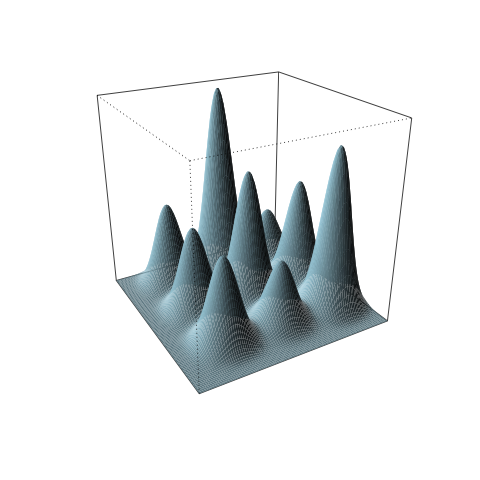
\includegraphics[width=4cm]{large-col-penalty}
% \caption{\small Strong column penalty}
% \end{figure}
%     \end{center}
%\end{column}
%\end{columns}
%

 





 
\section{\emph{``Unfold'' the two dimensional surface:}}

via the \emph{kronecker product}:
\begin{align*} %\label{eq:rowwise-kronecker-product}
B &= B_l \square B_m \\
&= \left( B_m \otimes 1^\prime_{K} \right) \odot \left(1^\prime_{L} \otimes  B_l  \right)\\
P_l  &=  I_L \otimes D_{d_{\ms l}}^\prime D_{d_{\ms l}}\\
P_m &=   D_{d_{\ms m}}^\prime D_{d_{\ms m}} \otimes I_K
\end{align*}
to write
\begin{equation*}
\mbox{vec}\left\{ \phi^*\left(l,m\right)\right \} = B \theta
\end{equation*}

 




 
\section{\emph{Then the penalized likelihood has convenient form:}}

\begin{equation*} %\label{eq:tensor-pspline-objective-function}
Q = \left( Y - WB\theta\right)^\prime D^{-1} \left( Y - WB\theta\right) + \lambda_l  \theta^\prime P_l \theta + \lambda_m \theta^\prime P_m \theta 
\end{equation*}


\begin{align*} \label{eq:tensor-pspline-normal-equations}
\hat{\theta}_\lambda = \left[ \left(WB\right)^\prime D^{-1}WB +  \lambda_l P_l+ \lambda_m P_m\right]^{-1} \left(W B\right)^\prime Y
\end{align*}
Degrees of freedom can be approximated as in the usual smoothing case:
\begin{align*}
\textup{ED} &= \textup{tr} \left[ H_\lambda \right]\\
&= \textup{tr}\bigg[\left[ \left(WB\right)^\prime D^{-1}WB +  \lambda_l P_l+ \lambda_m P_m\right]^{-1} \left(W B\right)^\prime WB  \bigg]
\end{align*}

AIC, GCV, CV accessible for model diagnostics.

 


\subsection{Banding the Cholesky factor}

A recent upsurge in the application of regularization to large empirical covariance matrices includes the work \citet{huang2006covariance}, \citet{furrer2007estimation}, \citet{fan2008high}, \citet{ledoit2004well}.  \citet{furrer2007estimation} propose stabilizing the sample covariance matrix by ``tapering,'' or gradually shrinking the off-diagonal elements to zero. \citet{d2008first} propose a sparse estimator by applying an $L_1$ penalty directly to the elements of the covariance matrix. Instead of regularizing the covariance matrix itself, some have opted to regularize its inverse;  \cite{wu2003nonparametric} band the Cholesky decomposition  by setting certain diagonals of the Cholesky factor to zero. \citet{huang2006covariance} and \citet{levina2008sparse} use $L_1$ penalties to achieve parsimony of the entries of the Cholesky factor; sparsity of the Cholesky factor, however, does not necessarily imply sparsity in the inverse covariance matrix. \citet{levina2008sparse} propose banding the Cholesky factor using a nested Lasso penalty which yields sparse estimators of the precision matrix.  

\cite{pourahmadi1999joint} presented a hueristic argument that the GARPs, $\phi_{t,t-l}$ should be monotonically decreasing in absolute value as $l$ increases. The following proposition establishes the relationship between zeros in the Cholesky factor and zeroes in the inverse covariance, connecting the regularization of $\phi^*$  to the structure in the resulting inverse covariance matrix. 

\begin{proposition} \label{prop:cholesky-inverse-banding-equivalence}
Let $\Omega$ denote a $m \times m$ positive definite matrix with elements $\omega_{ij}$ with modified Cholesky decomposition $T^\prime D^{-1} T$, where $T$ is unit lower triangular. Let  $t_{ij}$ denote the $ij^{th}$ element of $T$. For any column $j$ and row $r\left(j\right) > j$,  $\omega_{mj} = \dots = \omega_{r\left(j\right),j} = 0$ if and only if  $t_{mj} = \dots = t_{r\left(j\right),j} = 0$.
\end{proposition}


The proof is left to the appendix. Proposition~\ref{prop:cholesky-inverse-banding-equivalence} maintains that the modified Cholesky factor $T$ with arbitrary column band lengths corresponds to inverse covariance matrix $\Omega$ with the same column band lengths, and hence the inverse covariance matrix is $K$-banded if and only if its Cholesky factor is $K$-banded. That is, if $\phi^*$ is zero or nearly zero for  large $\vert i-j \vert$, then $y_i$ and $y_j$ are conditionally uncorrelated (or nearly so). This suggests that the effect of $y_{t-l}$ on $y_t$ through model~\ref{eq:MyModel} should decrease as the time between the two measurements increases, such that
 
\[
\phi^*\left(l,m\right) \approx 0
\]
\noindent
for large $l$ is a reasonable way to institute regularization. 


This notion of sparsity is quite different from the notion of smoothness imposed by the usual derivative-based penalties or the analog difference penalties for P-splines; however, the local support of the B-spline basis functions permits the intuitive expression of a penalty to be used for banding the Cholesky factor. The B-spline basis functions are non-negative on their support; therefore, if a B-spline (as in \ref{eq:b-spline-representation}) is zero for $l > l_0$, then the coefficients of the B-splines contributing to that region of the domain are also zero. For functions represented using order $k$ B-spline basis functions $\lbrace B_i \rbrace$, $i=1,\dots,n$, one may truncate the function to zero at some truncation point $l_0 \in \left(0,1\right)$ by penalizing the size of the coefficients corresponding to any basis functions having support on $l > l_0$. This naturally leads to penalties of the form

\begin{equation} \label{eq:banded-pspline-penalty}
J_{B} = \sum_{ i=i^* -k }^n \vert \theta_i \vert^p
\end{equation}
\noindent
where
\[
i^* = \max\limits_{i} \left\{ \ell_i: \ell_i \le l_0 \right\}
\]
is the index of the largest knot which is smaller than the truncation point $l_0$. Setting $p=1$ in \ref{eq:banded-pspline-penalty} corresponds to putting a LASSO penalty (see \citet{tibshirani1996regression}) on the coefficients contributing to the function value on $l > l_0$, while setting $p=2$ corresponds to the usual ridge regression setting. 


Several have proposed regularization of the inverse covariance matrix by ``banding'' the Cholesky factor $T$: setting all elements of $T$ beyond the $K^{th}$ off-diagonal to zero, i.e. setting $\phi_{t,t-l}=0$ for $l > K$ for some choice of $K$.  (See \cite{pourahmadi1999joint}, \citet{wu2003nonparametric}, \cite{bickel2008regularized}, and \cite{huang2007estimation}.) In terms of model~\ref{eq:ARmodel}, this is equivalent to regressing $y_t$  on only its $K$ immediate predecessors, setting the regression coefficient for $y_{t-l}$ to zero for $l>K$.  This notion is instrumental in justifying a family of penalties which induces an alternative decomposition of the function space for which the null space of these penalties comprises functions $\phi^*$ taking nonzero values on a subset of the domain:

\begin{equation} \label{eq:banded-penalty-nullspace}
\mathcal{H}_0\left(\mathcal{B}\right) = \left\{ \phi^*: \phi^*\left(l,m\right) = 0 \mbox{ for all } l > l_0 \right\},
\end{equation}
\noindent
which is equivalent to the set of functions having compact support:

\[
supp\left( \phi^* \right) = \left(0,l_0\right].
\]

 



 
\section{\emph{Recap: from the top}}

\begin{itemize}
\item We propose a general framework for unconstrained covariance estimation.
\item Flexibility permits imposing various types of regularization with ease. 
\item Penalty specification is crucial for performance.
\end{itemize}

 



 
\section{What's next?}

\begin{itemize}
\item ``designer'' penalties - impose desirable shape constraints (decay in $l$)
\item Additive, ANOVA models for $\phi^*$
\item P-spline model reparameterized as mixture models
\end{itemize}

 



%
%\begin{equation*}
%P  = \begin{bmatrix}
%0 &&&\\
%& \underbracket[0.2pt]{\lambda_l D_{\ms{d_l}}^\prime D_{\ms{d_l}}}_{\text{$P_{\ms l}$}}	& 	& \\
%&&& \\
%&	&	\underbracket[0.2pt]{\lambda_l D_{\ms{d_l}}^\prime D_{\ms{d_l}}}_{\text{$P_{\ms m}$}}	& 	\\
%&&&\\
%&&&	\underbracket[0.2pt]{\tau_m D_{\ms{d_m}}^\prime D_{\ms{d_m}} \otimes I_{\ms{c_l}} + \tau_l I_{\ms{c_m}} \otimes D_{\ms{d_l}}^\prime D_{\ms{d_l}}}_{\text{$P_{\ms lm}$}}
%\end{bmatrix}
%\end{equation*}
%
% 



%
%
%%% NEEDS CORRECTED TO ACCOUNT FOR REPLACING \sigma^2 I with D
%
% 
%\section{\emph{Mixed model representation}}
%
%Find orthogonal transformation $\mathrm{Q} = \left[\begin{array}{c|c} \mathrm{Q}_0 & \mathrm{Q}_1 \end{array}\right]$; map
%%\begin{equation*}
%%\newmaththought{B} \longrightarrow \mixedmodelmath{ \big[ \begin{array}{c|c} X & Z \end{array}  \big]}, \qquad \newmaththought{\theta} \longrightarrow \mixedmodelmath{\left( \beta^\prime, \alpha^\prime \right)^\prime}
%%\end{equation*}
%%\noindent
%%such that 
%
%\begin{align*}
%BQ &=\mixedmodelmath{ \big[ \begin{array}{c|c} B\mathrm{Q}_{\ms 0} &  B\mathrm{Q}_{\ms 1} \end{array}  \big]}	\\	
%&=  \mixedmodelmath{ \big[ \begin{array}{c|c} X & Z \end{array}  \big]}\\
%\end{align*}
%\noindent
%such that
%\begin{equation*}
%B\theta = \mixedmodelmath{X\beta + Z\alpha}
%\end{equation*}
%
%
%
%Model~\ref{eq:PS-ANOVA} becomes
%\begin{equation} \label{eq:vc-mixed-effects-model}
%Y = W\left(X \beta + Z \alpha\right) + e 
%\end{equation}
%\begin{equation*}
% \alpha \sim \mathcal{N}\left(0,G \right), \quad
% e\sim\mathcal{N}\left(0, \sigma_{\ms e}^2 D \right)
%\end{equation*}
%
%
%
% 
%
%
%


%
%
% 
%\section{\emph{Nested B-spline bases}}
%
%For $d_{\ms l} = d_{\ms m} = 2$, 
%\begin{align*} 
%X &= \left[\begin{array}{c|c|c|c} 1 & 1 \square l & m \square 1 & m \square l  \end{array} \right] \\
%Z &= \left[\begin{array}{c|c|c|c|c} 1 \square Z_{\ms l}& Z_{\ms m} \square 1 & m \square  Z_{\ms l} &  Z_{\ms m} \square l &  Z_{\ms m} \square  Z_{\ms l}\end{array} \right] 
%\end{align*} 
%
%
%\begin{align*}
% \phi_{\ms{12}}\left(l,m\right)  =   \sum_{r=1}^{\ms{d_m-1}} m^{\ms r}g_{\ms lr}\left(l\right) +  \sum_{r^\prime=1}^{\ms{d_l-1}} l^{\ms r^\prime}  g_{\ms mr^\prime}\left(m\right)+ h\left( l,m \right),
%\end{align*}
%\noindent
%For $d_l = d_m = 2$,
%\[
% \phi_{\ms{12}}\left(l,m\right)  = g_{\ms 1}\left(l\right) \; m+ l \; g_{\ms 2}\left(m\right) + \; h\left( l,m \right) 
%\]
%
%%\begin{equation} \label{eq:nested-SANOVA-basis-matrix}
%%B = \big[  \; 1 \; \vert \;  B_1  \; \vert \;   B_2 \; \vert  B_3 \; \vert B_4 \; \vert B_5 \; \big],
%%\end{equation}
%%\noindent
%%where
%%\[
%%\begin{array}{ccc}
%%B_{\ms 3} = m \; \square \;  B_{\ms 1}, \;\; & B_{\ms 4}  = B_{\ms 2}  \square \; l, \;\; &  B_{\ms 5}= B_{\ms 2} \;\square \; B_{\ms 1} 
%%\end{array}
%%\]
%%\begin{equation*} \label{eq:PSANOVA-penalty}
%%P = \mbox{blockdiag}\left(0,\; P_1, \; P_2, \; P_{3},\; P_4, \; P_{5} \right),
%%\end{equation*}
%
% 


%
%
%
% 
%\section{\emph{\normalsize{Smoothing parameter selection = variance component estimation}}}
%
%\vspace{0.2in}
%$G = \sigma_{\ms e}^2 F^{-1}$ where
%
%\begin{align*}
%F &= \left[\begin{array}{ccc}
%F_{\ms l} &&\\
%&F_{\ms m} &\\
%&& F_{\ms lm}\\
%\end{array}\right]
% = \left[\begin{array}{ccc}
%\lambda_l \tilde{\Delta}_l &&\\
%&\lambda_m \tilde{\Delta}_m &\\
%&& F_{\ms lm}\\
%\end{array}\right],
%\end{align*}
%%
%
%\begin{equation*}
% F_{\ms lm} = \left[\begin{array}{ccc}
%\tau_l \tilde{\Delta}_l &&\\
%&&\\
%&\tau_m \tilde{\Delta}_m&\\
%&&\\
%&&\tau_m \tilde{\Delta}_m \otimes I_{\ms{c_l-d_l}} +  I_{\ms{c_m-d_m}} \otimes \tau_l \tilde{\Delta}_l \end{array}\right]
%\end{equation*}
%
%
% 
%
%











% 
%\section{\emph{Decomposition of} $\phi^*$ \emph{for} $d_l = d_m = 2$}
%
%%This slide will decompose the function into its parametric and nonparametric components [add a (d_l + 1) x (d_m + 1) two way table with the decompositions of the marginal bases across the margins ]
%
%\begin{table}[h]
%%\caption{Decomposition of \phi^* for $d_l = d_m = 2$} %title of the table
%\centering % centering table
%\begin{tabular}{c|ccccc}
%	&    $\left\{ 1 \right\}$	&&	$\left\{m \right\}$	 	&& 	$\left\{ B_{\ms{j^\prime}}\left(m\right) \right\} $ \\ [0.5ex]
%\hline % inserts single-line
%\\
%$\left\{ 1 \right\}$ 				&  $\left\{ 1 \right\}$   	& &	$\left\{m \right\}$	 	&& 	$\left\{ B_{\ms{j^\prime}}\left(m\right) \right\} $	\\  [2.5ex] % Entering row contents
%$\left\{l \right\}$		 		&  $\left\{ l \right\}$  	 &&	$l \times m$	 	&& 	$l \times \left\{   B_{\ms{j^\prime}}\left(m\right) \right\} $\\  [2.5ex]
%$\left\{ B_j\left(l\right) \right\} $	 	&    $\left\{ B_j\left(l\right) \right\}$	&&	$ m \times \left\{ B_j\left(l\right) \right\}$	& &	$\left\{ B_j\left(l\right) B_{\ms{j^\prime}}\left(m\right) \right\}$ 
%\end{tabular}
%\end{table}
%
% 




%
% 
%\section{\emph{Now the variance components have simpler structure.}}
%
%Let $\alpha_k \sim \mathcal{N}\left(0,G_k\right)$,
%\begin{align*}
%Z &= \left[\begin{array}{c|c|c|c|c} Z_1 & Z_2 & Z_3 & Z_4 & Z_5\end{array} \right]\\
%&= \left[\begin{array}{c|c|c|c|c} \coolunderbrace{\alpha_1}{1 \square Z_{\ms l}}  & \coolunderbrace{\alpha_2}{Z_{\ms m} \square 1} & \coolunderbrace{\alpha_3}{m \square  Z_{\ms l}} & \coolunderbrace{\alpha_4}{ Z_{\ms m} \square l} &  \coolunderbrace{\alpha_5}{Z_{\ms m} \square  Z_{\ms l} } \end{array} \right]
%\end{align*}
%
%\vspace{0.2in}
%Take $Z_k^* = Z_k F_k^{-1}$, then
%
%\begin{align*}
%G  &= \mbox{blockdiag}\left(G_1,\;G_2,\;G_3,\;G_4,\;G_5 \right)\\
%  &= \mbox{blockdiag}\left(\tau_1^2 I_{{\ms c_l - 2}},\; \tau_2^2 I_{{\ms c_m - 2}},\;\tau_3^2 I_{{\ms c_l - 2}},\;\tau_4^2 I_{{\ms c_m - 2}},\;\tau_5^2 I_{{\ms \left(c_l - 2\right) \left(c_m - 2\right)}} \right)\\
%\end{align*}
%
% 
%
%


%
%
% 
%\section{REML for $\sigma_e^2$ and $\tau_k^2$ }
%
%Take $\hat{\tau}_k^2$, $\hat{\sigma}_e^2$ to be the minimizers of
%
%\begin{align*}
%\mathcal{L}=&-\frac{1}{2} \log \vert V \vert -\frac{1}{2} \log \vert X^\prime W^\prime V^{-1} W X \vert \\
%&-\frac{1}{2} y^\prime \left(V^{-1} - V^{-1}X^\prime W^\prime \left(X^\prime W^\prime V^{-1} WX \right)^{-1}X^\prime W^\prime  V^{-1} \right)y 
%\end{align*}
%
%where 
%\begin{equation}
%V = Cov \left( Y \right) = \sigma_e^2 D + WZGZ^\prime W^\prime
%\end{equation}
% 






% 
%\section{REML for $\sigma_e^2$ and $\tau_k^2$ }
%
%Take $\hat{\sigma}_e^2$, $\hat{\tau}_k^2$ to minimize
%\begin{align*}
%-2\mathcal{L}= n \log \sigma_e &+ \sum_{j=1}^5 \left( k_j \log \tau_j + \log \sigma_e + \frac{\alpha_j^\prime \alpha_j}{\tau_j^2}\right)  \\[5pt]
%&+ \sigma_e^{-2}\left(Y - W\left(X\beta - Z\alpha \right) \right)^\prime  \left(Y - W\left(X\beta - Z\alpha \right) \right) 
%\end{align*}
%
%
%\begin{align*}
%\hat{\tau}_k^2 &=  \frac{\hat{\alpha}_k^\prime\hat{\alpha}_k}{  \textup{ED}_j}, \\
% \hat{\sigma}_e^2 &= \frac{\left(Y - W\left(X\hat{\beta} - Z\hat{\alpha}\right) \right)^\prime  \left(Y - W\left(X\hat{\beta} - Z\hat{\alpha}\right) \right)}{N - \textup{ED}}
%\end{align*}
% 
%
%
%



%
% 
%
%\section{Appendix}
%
%\begin{align*}
%B_{\ms{lm}} &= B_m \; \square \; B_l \\   
%&\equiv \left( B_m \otimes 1^\prime_{c_l} \right) \odot \left(1^\prime_{c_m} \otimes  B_l  \right)    
%\end{align*}
%
%
%\begin{align*}
%\textup{ED} = \textup{trace}\left( H \right) = \textup{trace}\bigg[\left(\left[X\;Z \right]^\prime\left[X\;Z \right] + \mathring{G} \right)^{-1} \left[X\;Z \right]^\prime\left[X\;Z \right] \bigg] 
%\end{align*}
%
%
% 
%


\bibliography{Master}
\end{document}
